\documentclass[]{book}
\usepackage{lmodern}
\usepackage{amssymb,amsmath}
\usepackage{ifxetex,ifluatex}
\usepackage{fixltx2e} % provides \textsubscript
\ifnum 0\ifxetex 1\fi\ifluatex 1\fi=0 % if pdftex
  \usepackage[T1]{fontenc}
  \usepackage[utf8]{inputenc}
\else % if luatex or xelatex
  \ifxetex
    \usepackage{mathspec}
  \else
    \usepackage{fontspec}
  \fi
  \defaultfontfeatures{Ligatures=TeX,Scale=MatchLowercase}
\fi
% use upquote if available, for straight quotes in verbatim environments
\IfFileExists{upquote.sty}{\usepackage{upquote}}{}
% use microtype if available
\IfFileExists{microtype.sty}{%
\usepackage{microtype}
\UseMicrotypeSet[protrusion]{basicmath} % disable protrusion for tt fonts
}{}
\usepackage[margin=1in]{geometry}
\usepackage{hyperref}
\hypersetup{unicode=true,
            pdftitle={A Minimal Book Example},
            pdfauthor={Yihui Xie},
            pdfborder={0 0 0},
            breaklinks=true}
\urlstyle{same}  % don't use monospace font for urls
\usepackage{natbib}
\bibliographystyle{apalike}
\usepackage{color}
\usepackage{fancyvrb}
\newcommand{\VerbBar}{|}
\newcommand{\VERB}{\Verb[commandchars=\\\{\}]}
\DefineVerbatimEnvironment{Highlighting}{Verbatim}{commandchars=\\\{\}}
% Add ',fontsize=\small' for more characters per line
\usepackage{framed}
\definecolor{shadecolor}{RGB}{248,248,248}
\newenvironment{Shaded}{\begin{snugshade}}{\end{snugshade}}
\newcommand{\KeywordTok}[1]{\textcolor[rgb]{0.13,0.29,0.53}{\textbf{#1}}}
\newcommand{\DataTypeTok}[1]{\textcolor[rgb]{0.13,0.29,0.53}{#1}}
\newcommand{\DecValTok}[1]{\textcolor[rgb]{0.00,0.00,0.81}{#1}}
\newcommand{\BaseNTok}[1]{\textcolor[rgb]{0.00,0.00,0.81}{#1}}
\newcommand{\FloatTok}[1]{\textcolor[rgb]{0.00,0.00,0.81}{#1}}
\newcommand{\ConstantTok}[1]{\textcolor[rgb]{0.00,0.00,0.00}{#1}}
\newcommand{\CharTok}[1]{\textcolor[rgb]{0.31,0.60,0.02}{#1}}
\newcommand{\SpecialCharTok}[1]{\textcolor[rgb]{0.00,0.00,0.00}{#1}}
\newcommand{\StringTok}[1]{\textcolor[rgb]{0.31,0.60,0.02}{#1}}
\newcommand{\VerbatimStringTok}[1]{\textcolor[rgb]{0.31,0.60,0.02}{#1}}
\newcommand{\SpecialStringTok}[1]{\textcolor[rgb]{0.31,0.60,0.02}{#1}}
\newcommand{\ImportTok}[1]{#1}
\newcommand{\CommentTok}[1]{\textcolor[rgb]{0.56,0.35,0.01}{\textit{#1}}}
\newcommand{\DocumentationTok}[1]{\textcolor[rgb]{0.56,0.35,0.01}{\textbf{\textit{#1}}}}
\newcommand{\AnnotationTok}[1]{\textcolor[rgb]{0.56,0.35,0.01}{\textbf{\textit{#1}}}}
\newcommand{\CommentVarTok}[1]{\textcolor[rgb]{0.56,0.35,0.01}{\textbf{\textit{#1}}}}
\newcommand{\OtherTok}[1]{\textcolor[rgb]{0.56,0.35,0.01}{#1}}
\newcommand{\FunctionTok}[1]{\textcolor[rgb]{0.00,0.00,0.00}{#1}}
\newcommand{\VariableTok}[1]{\textcolor[rgb]{0.00,0.00,0.00}{#1}}
\newcommand{\ControlFlowTok}[1]{\textcolor[rgb]{0.13,0.29,0.53}{\textbf{#1}}}
\newcommand{\OperatorTok}[1]{\textcolor[rgb]{0.81,0.36,0.00}{\textbf{#1}}}
\newcommand{\BuiltInTok}[1]{#1}
\newcommand{\ExtensionTok}[1]{#1}
\newcommand{\PreprocessorTok}[1]{\textcolor[rgb]{0.56,0.35,0.01}{\textit{#1}}}
\newcommand{\AttributeTok}[1]{\textcolor[rgb]{0.77,0.63,0.00}{#1}}
\newcommand{\RegionMarkerTok}[1]{#1}
\newcommand{\InformationTok}[1]{\textcolor[rgb]{0.56,0.35,0.01}{\textbf{\textit{#1}}}}
\newcommand{\WarningTok}[1]{\textcolor[rgb]{0.56,0.35,0.01}{\textbf{\textit{#1}}}}
\newcommand{\AlertTok}[1]{\textcolor[rgb]{0.94,0.16,0.16}{#1}}
\newcommand{\ErrorTok}[1]{\textcolor[rgb]{0.64,0.00,0.00}{\textbf{#1}}}
\newcommand{\NormalTok}[1]{#1}
\usepackage{longtable,booktabs}
\usepackage{graphicx,grffile}
\makeatletter
\def\maxwidth{\ifdim\Gin@nat@width>\linewidth\linewidth\else\Gin@nat@width\fi}
\def\maxheight{\ifdim\Gin@nat@height>\textheight\textheight\else\Gin@nat@height\fi}
\makeatother
% Scale images if necessary, so that they will not overflow the page
% margins by default, and it is still possible to overwrite the defaults
% using explicit options in \includegraphics[width, height, ...]{}
\setkeys{Gin}{width=\maxwidth,height=\maxheight,keepaspectratio}
\IfFileExists{parskip.sty}{%
\usepackage{parskip}
}{% else
\setlength{\parindent}{0pt}
\setlength{\parskip}{6pt plus 2pt minus 1pt}
}
\setlength{\emergencystretch}{3em}  % prevent overfull lines
\providecommand{\tightlist}{%
  \setlength{\itemsep}{0pt}\setlength{\parskip}{0pt}}
\setcounter{secnumdepth}{5}
% Redefines (sub)paragraphs to behave more like sections
\ifx\paragraph\undefined\else
\let\oldparagraph\paragraph
\renewcommand{\paragraph}[1]{\oldparagraph{#1}\mbox{}}
\fi
\ifx\subparagraph\undefined\else
\let\oldsubparagraph\subparagraph
\renewcommand{\subparagraph}[1]{\oldsubparagraph{#1}\mbox{}}
\fi

%%% Use protect on footnotes to avoid problems with footnotes in titles
\let\rmarkdownfootnote\footnote%
\def\footnote{\protect\rmarkdownfootnote}

%%% Change title format to be more compact
\usepackage{titling}

% Create subtitle command for use in maketitle
\newcommand{\subtitle}[1]{
  \posttitle{
    \begin{center}\large#1\end{center}
    }
}

\setlength{\droptitle}{-2em}
  \title{A Minimal Book Example}
  \pretitle{\vspace{\droptitle}\centering\huge}
  \posttitle{\par}
  \author{Yihui Xie}
  \preauthor{\centering\large\emph}
  \postauthor{\par}
  \predate{\centering\large\emph}
  \postdate{\par}
  \date{2017-09-24}

\usepackage{booktabs}
\usepackage{amsthm}
\makeatletter
\def\thm@space@setup{%
  \thm@preskip=8pt plus 2pt minus 4pt
  \thm@postskip=\thm@preskip
}
\makeatother

\usepackage{amsthm}
\newtheorem{theorem}{Theorem}[chapter]
\newtheorem{lemma}{Lemma}[chapter]
\theoremstyle{definition}
\newtheorem{definition}{Definition}[chapter]
\newtheorem{corollary}{Corollary}[chapter]
\newtheorem{proposition}{Proposition}[chapter]
\theoremstyle{definition}
\newtheorem{example}{Example}[chapter]
\theoremstyle{definition}
\newtheorem{exercise}{Exercise}[chapter]
\theoremstyle{remark}
\newtheorem*{remark}{Remark}
\newtheorem*{solution}{Solution}
\begin{document}
\maketitle

{
\setcounter{tocdepth}{1}
\tableofcontents
}
\chapter{Prerequisites}\label{prerequisites}

This is a \emph{sample} book written in \textbf{Markdown}. You can use
anything that Pandoc's Markdown supports, e.g., a math equation
\(a^2 + b^2 = c^2\).

For now, you have to install the development versions of
\textbf{bookdown} from Github:

\begin{Shaded}
\begin{Highlighting}[]
\NormalTok{devtools}\OperatorTok{::}\KeywordTok{install_github}\NormalTok{(}\StringTok{"rstudio/bookdown"}\NormalTok{)}
\end{Highlighting}
\end{Shaded}

Remember each Rmd file contains one and only one chapter, and a chapter
is defined by the first-level heading \texttt{\#}.

To compile this example to PDF, you need to install XeLaTeX.

\chapter{Introduction}\label{intro}

You can label chapter and section titles using \texttt{\{\#label\}}
after them, e.g., we can reference Chapter \ref{intro}. If you do not
manually label them, there will be automatic labels anyway, e.g.,
Chapter \ref{methods}.

Figures and tables with captions will be placed in \texttt{figure} and
\texttt{table} environments, respectively.

\begin{Shaded}
\begin{Highlighting}[]
\KeywordTok{par}\NormalTok{(}\DataTypeTok{mar =} \KeywordTok{c}\NormalTok{(}\DecValTok{4}\NormalTok{, }\DecValTok{4}\NormalTok{, .}\DecValTok{1}\NormalTok{, .}\DecValTok{1}\NormalTok{))}
\KeywordTok{plot}\NormalTok{(pressure, }\DataTypeTok{type =} \StringTok{'b'}\NormalTok{, }\DataTypeTok{pch =} \DecValTok{19}\NormalTok{)}
\end{Highlighting}
\end{Shaded}

\begin{figure}

{\centering 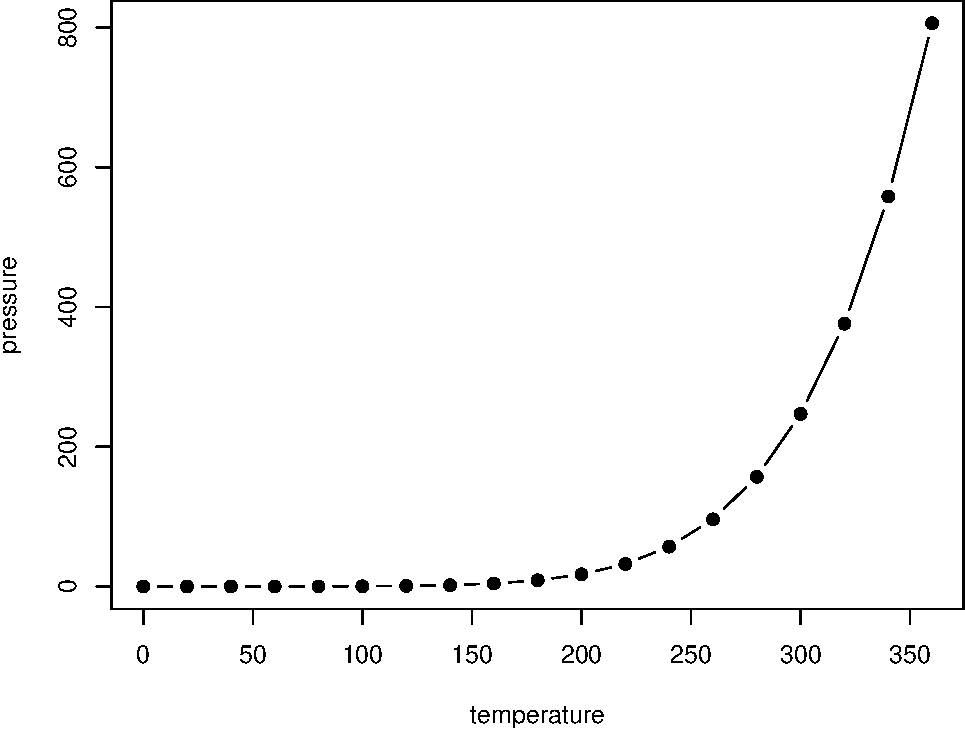
\includegraphics[width=0.8\linewidth]{bookdown-demo_files/figure-latex/nice-fig-1} 

}

\caption{Here is a nice figure!}\label{fig:nice-fig}
\end{figure}

Reference a figure by its code chunk label with the \texttt{fig:}
prefix, e.g., see Figure \ref{fig:nice-fig}. Similarly, you can
reference tables generated from \texttt{knitr::kable()}, e.g., see Table
\ref{tab:nice-tab}.

\begin{Shaded}
\begin{Highlighting}[]
\NormalTok{knitr}\OperatorTok{::}\KeywordTok{kable}\NormalTok{(}
  \KeywordTok{head}\NormalTok{(iris, }\DecValTok{20}\NormalTok{), }\DataTypeTok{caption =} \StringTok{'Here is a nice table!'}\NormalTok{,}
  \DataTypeTok{booktabs =} \OtherTok{TRUE}
\NormalTok{)}
\end{Highlighting}
\end{Shaded}

\begin{table}

\caption{\label{tab:nice-tab}Here is a nice table!}
\centering
\begin{tabular}[t]{rrrrl}
\toprule
Sepal.Length & Sepal.Width & Petal.Length & Petal.Width & Species\\
\midrule
5.1 & 3.5 & 1.4 & 0.2 & setosa\\
4.9 & 3.0 & 1.4 & 0.2 & setosa\\
4.7 & 3.2 & 1.3 & 0.2 & setosa\\
4.6 & 3.1 & 1.5 & 0.2 & setosa\\
5.0 & 3.6 & 1.4 & 0.2 & setosa\\
\addlinespace
5.4 & 3.9 & 1.7 & 0.4 & setosa\\
4.6 & 3.4 & 1.4 & 0.3 & setosa\\
5.0 & 3.4 & 1.5 & 0.2 & setosa\\
4.4 & 2.9 & 1.4 & 0.2 & setosa\\
4.9 & 3.1 & 1.5 & 0.1 & setosa\\
\addlinespace
5.4 & 3.7 & 1.5 & 0.2 & setosa\\
4.8 & 3.4 & 1.6 & 0.2 & setosa\\
4.8 & 3.0 & 1.4 & 0.1 & setosa\\
4.3 & 3.0 & 1.1 & 0.1 & setosa\\
5.8 & 4.0 & 1.2 & 0.2 & setosa\\
\addlinespace
5.7 & 4.4 & 1.5 & 0.4 & setosa\\
5.4 & 3.9 & 1.3 & 0.4 & setosa\\
5.1 & 3.5 & 1.4 & 0.3 & setosa\\
5.7 & 3.8 & 1.7 & 0.3 & setosa\\
5.1 & 3.8 & 1.5 & 0.3 & setosa\\
\bottomrule
\end{tabular}
\end{table}

You can write citations, too. For example, we are using the
\textbf{bookdown} package \citep{R-bookdown} in this sample book, which
was built on top of R Markdown and \textbf{knitr} \citep{xie2015}.

\chapter{Linear Regression with One
Regressor}\label{linear-regression-with-one-regressor}

This chapter introduces the simple linear regression model which relates
one variable, \(X\), to another variable \(Y\). If for example a school
cuts the class sizes by hiring new teachers, that is the school lowers
the student-teacher ratios of their classes, how would this effect the
performance of the students? With linear regression we can not only
examine whether the student-teacher ratio \(\left(X\right)\) does have
an impact on the test results \(\left(Y\right)\). We can also learn
about the direction and the strength of this effect.

To start with an easy example, consider the following combinations of
average test score and the average student-teacher ratio of some
fictional classes.

\begin{longtable}[]{@{}llllllll@{}}
\toprule
& 1 & 2 & 3 & 4 & 5 & 6 & 7\tabularnewline
\midrule
\endhead
Test Score & 680 & 640 & 670 & 660 & 630 & 660 & 635\tabularnewline
STR & 15 & 17 & 19 & 20 & 22 & 23.5 & 25\tabularnewline
\bottomrule
\end{longtable}

To work with this data in R, we create 2 vectors, one for the
student-teacher ratios and one for test scores which contain the data
from the table above.

\begin{Shaded}
\begin{Highlighting}[]
\CommentTok{# Create sample data}
\NormalTok{STR <-}\StringTok{ }\KeywordTok{c}\NormalTok{(}\DecValTok{15}\NormalTok{, }\DecValTok{17}\NormalTok{, }\DecValTok{19}\NormalTok{, }\DecValTok{20}\NormalTok{, }\DecValTok{22}\NormalTok{, }\FloatTok{23.5}\NormalTok{, }\DecValTok{25}\NormalTok{)}
\NormalTok{TestScore <-}\StringTok{ }\KeywordTok{c}\NormalTok{(}\DecValTok{680}\NormalTok{, }\DecValTok{640}\NormalTok{, }\DecValTok{670}\NormalTok{, }\DecValTok{660}\NormalTok{, }\DecValTok{630}\NormalTok{, }\DecValTok{660}\NormalTok{, }\DecValTok{635}\NormalTok{) }

\CommentTok{# Print out sample data}
\NormalTok{STR}
\end{Highlighting}
\end{Shaded}

\begin{verbatim}
## [1] 15.0 17.0 19.0 20.0 22.0 23.5 25.0
\end{verbatim}

\begin{Shaded}
\begin{Highlighting}[]
\NormalTok{TestScore}
\end{Highlighting}
\end{Shaded}

\begin{verbatim}
## [1] 680 640 670 660 630 660 635
\end{verbatim}

If we use a simple linear regression model, we assume that the true
relationship between both variables can be represented by a straight
line, formally

\[ y = bx + a. \]

Let us suppose that the true function which relates test score and
student-teacher ratio to each other is

\[TestScore = 713 - 3 \times STR.\]

If possible, it is always a good idea to visualize the data You work
with in an appropriate way. For our purpose it is suitable to use the
function \texttt{plot()} to produce a scatterplot with \texttt{STR} on
the \(X\)-axis and \texttt{TestScore} on the \(Y\)-axis. An easy way to
do so is to call
\texttt{plot(y\_variable\ \textasciitilde{}\ x\_variable)} whereby
\texttt{y\_variable} and \texttt{x\_variable} are placeholders for the
vectors of observations we want to plot. Furthermore, we might want to
add the true relationship to the plot. To draw a straight line, R
provides the function \texttt{abline()}. We just have to call this
function with arguments \texttt{a} (representing the intercept) and
\texttt{b} (representing the slope) after executing \texttt{plot()} in
order to add the line to our scatterplot. The following code reproduces
figure 4.1 from the textbook.

\begin{Shaded}
\begin{Highlighting}[]
\CommentTok{# create a scatter plot of the data}
\KeywordTok{plot}\NormalTok{(TestScore }\OperatorTok{~}\StringTok{ }\NormalTok{STR)}

\CommentTok{# add the true relationship to the plot}
\KeywordTok{abline}\NormalTok{(}\DataTypeTok{a =} \DecValTok{713}\NormalTok{, }\DataTypeTok{b =} \OperatorTok{-}\DecValTok{3}\NormalTok{)}
\end{Highlighting}
\end{Shaded}

\begin{center}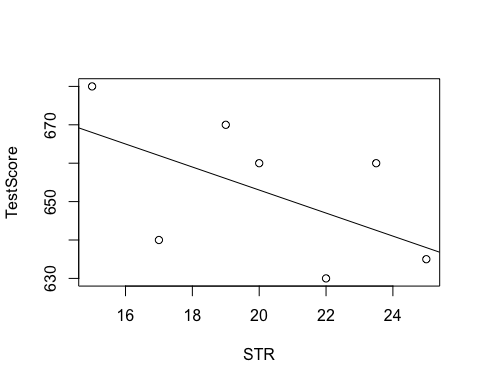
\includegraphics{bookdown-demo_files/figure-latex/Figure 4.1-1} \end{center}

We find that our line does not touch any of the points although we
claimed that it represents the true relationship. The reason for this is
the core problem of statistics, randomness. Most of the time there are
influences which cannot be explained in a purely deterministic fashion
and thus exacerbate finding of the true relationship.

In order to account for these differences between observed data and the
true relationship, we extend our model from above by an \emph{error
term} \(u\) which covers these random effects. Put differently, \(u\)
accounts for all the differences between the true regression line and
the actual observed data. Beside pure randomness, these deviations could
also arise from measerment errors or, as will be discussed later, are
the consequence of leaving out other factors that are relevant in
explaining the dependent variable. Which other factor are plausible in
our example? For one thing, the test scores might be driven by the
teachers quality and the background of the students. It is also
imaginable that in some classes, the students were lucky on the test
days and thus achieved higher scores. For now, we will summarize such
influences by an additive component:

\[ TestScore = \beta_0 + \beta_1 \times STR + \text{other factors} \]

Of course this idea is very general as it can be easily extented to
other situations that can be described with a linear model. The basic
linear regression function we will work with hence is

\[ Y_i = \beta_0 + \beta_1 X_i + u_i. \]

Key Concept 4.1 summarizes the terminology of the simple linear
regression model.

Key Concept 4.1

Terminology for the Linear Regression Model with a Single Regressor

The linear regression model is

\[Y_i = \beta_0 + \beta_1 X_1 + u_i \]

where

\begin{itemize}
\tightlist
\item
  the subscript \(i\) runs over the observations, \(i = 1\), \ldots{},
  \(n\)
\item
  \(Y_i\) is the \emph{dependent variable}, the \emph{regressand}, or
  simply the \emph{left-hand variable}
\item
  \(X_i\) is the \emph{independent variable}, the \emph{regressor}, or
  simply the \emph{right-hand variable}
\item
  \(Y = \beta_0 + \beta_1 X\) is the \emph{population regression line}
  also called the \emph{population regression function}
\item
  \(\beta_0\) is the \emph{intercept} of the population regression line
\item
  \(\beta_1\) is the \emph{slope} of the population regression line
\item
  \(u_i\) is the \emph{error term}
\end{itemize}

\section{Estimating the Coefficients of the Linear Regression
Model}\label{estimating-the-coefficients-of-the-linear-regression-model}

In practice, the intercept \(\beta_0\) and slope \(\beta_1\)of the
population regression line are unknown. Therefore, we must employ data
to estimate both unknown parameters. In the following a real world
example will be used to demonstrate how this is achieved. We want to
relate test scores to student-teacher ratios in \(420\) California
school destricts. The test score is the district-wide average of reading
and math scores for fifth graders. Again, the class size is measured as
the number of students divided by the number of teachers (the
student-teacher ratio). The California School dataset is available a R
package called AER, an acronym for
\href{https://cran.r-project.org/web/packages/AER/AER.pdf}{Applied
Econometrics with R}. After installing the package with
\texttt{install.packages("AER")} and attaching it with
\texttt{library("AER")} the dataset can be loaded using the
\texttt{data} function.

\begin{Shaded}
\begin{Highlighting}[]
\CommentTok{# load the AER package }
\KeywordTok{library}\NormalTok{(AER)   }

\CommentTok{# load the the data set in the workspace}
\KeywordTok{data}\NormalTok{(CASchools) }
\end{Highlighting}
\end{Shaded}

For several reasons it is interesting to know what kind of object we are
dealing with. \texttt{class(object\_name)} returns the type (class) of
an object. Depending on the class of an object several functions (such
as \texttt{plot} and \texttt{summary}) behave differently.

\begin{Shaded}
\begin{Highlighting}[]
\KeywordTok{class}\NormalTok{(CASchools)}
\end{Highlighting}
\end{Shaded}

\begin{verbatim}
## [1] "data.frame"
\end{verbatim}

It turns out that \texttt{CASchools} is of class \texttt{data.frame}
which is a convienient format to work with.

With help of the function \texttt{head} we get a first overview of our
data. This function shows only the first 6 rows of the data set which
prevents an overcrowded console output (hint: press ctrl + L to clear
the console). An alternative to \texttt{class} and \texttt{head} is
\texttt{str} which is deduced from `structure' and gives a comprehensive
overview of the object.

\begin{Shaded}
\begin{Highlighting}[]
\KeywordTok{head}\NormalTok{(CASchools)}
\end{Highlighting}
\end{Shaded}

\begin{verbatim}
##   district                          school  county grades students
## 1    75119              Sunol Glen Unified Alameda  KK-08      195
## 2    61499            Manzanita Elementary   Butte  KK-08      240
## 3    61549     Thermalito Union Elementary   Butte  KK-08     1550
## 4    61457 Golden Feather Union Elementary   Butte  KK-08      243
## 5    61523        Palermo Union Elementary   Butte  KK-08     1335
## 6    62042         Burrel Union Elementary  Fresno  KK-08      137
##   teachers calworks   lunch computer expenditure    income   english  read
## 1    10.90   0.5102  2.0408       67    6384.911 22.690001  0.000000 691.6
## 2    11.15  15.4167 47.9167      101    5099.381  9.824000  4.583333 660.5
## 3    82.90  55.0323 76.3226      169    5501.955  8.978000 30.000002 636.3
## 4    14.00  36.4754 77.0492       85    7101.831  8.978000  0.000000 651.9
## 5    71.50  33.1086 78.4270      171    5235.988  9.080333 13.857677 641.8
## 6     6.40  12.3188 86.9565       25    5580.147 10.415000 12.408759 605.7
##    math
## 1 690.0
## 2 661.9
## 3 650.9
## 4 643.5
## 5 639.9
## 6 605.4
\end{verbatim}

We find that the dataset consists of plenty of variables and most of
them are numeric. The two variables we are intersted in (i.e.~average
test score and the student-teacher ratio) are not included. However, it
is possible to calculate both from the provided data. To obtain the
student-teacher ratios, we divide the number of students by the number
of teachers. The avarage test score is the arithmetic mean of the test
score for reading and the score of the math test. The next code chunk
shows how the two variables can be constructed and how they are added to
the dataframe \texttt{CASchools}

\begin{Shaded}
\begin{Highlighting}[]
\NormalTok{CASchools}\OperatorTok{$}\NormalTok{STR <-}\StringTok{ }\NormalTok{CASchools}\OperatorTok{$}\NormalTok{students}\OperatorTok{/}\NormalTok{CASchools}\OperatorTok{$}\NormalTok{teachers     }
\NormalTok{CASchools}\OperatorTok{$}\NormalTok{score <-}\StringTok{ }\NormalTok{(CASchools}\OperatorTok{$}\NormalTok{read }\OperatorTok{+}\StringTok{ }\NormalTok{CASchools}\OperatorTok{$}\NormalTok{math)}\OperatorTok{/}\DecValTok{2}     
\end{Highlighting}
\end{Shaded}

If we run \texttt{head} again we would now find the two variables of
interest \texttt{STR} and \texttt{score} (check this!).

Table 4.1 from the text book summarizes the distribution of test scores
and student-teacher ratios. The functions \texttt{mean} (computes the
arithmetic mean of the provided numbers), \texttt{sd} (computes the
standard deviation), and \texttt{quantile} (returns a vector of the
specified quantiles) can be used to obtain the same results.

In order to have a nice display format we gather all the data after the
computation in a \texttt{data.frame} object named
\texttt{DistributionSummary}.

\begin{Shaded}
\begin{Highlighting}[]
\CommentTok{# compute sample averages}
\NormalTok{avg_STR <-}\StringTok{ }\KeywordTok{mean}\NormalTok{(CASchools}\OperatorTok{$}\NormalTok{STR) }
\NormalTok{avg_score <-}\StringTok{ }\KeywordTok{mean}\NormalTok{(CASchools}\OperatorTok{$}\NormalTok{score)}

\CommentTok{# compute standard deviations}
\NormalTok{sd_STR <-}\StringTok{ }\KeywordTok{sd}\NormalTok{(CASchools}\OperatorTok{$}\NormalTok{STR) }
\NormalTok{sd_score <-}\StringTok{ }\KeywordTok{sd}\NormalTok{(CASchools}\OperatorTok{$}\NormalTok{score)}

\CommentTok{# set up a vector of percentiles and compute the quantiles }
\NormalTok{quantiles <-}\StringTok{ }\KeywordTok{c}\NormalTok{(}\FloatTok{0.10}\NormalTok{, }\FloatTok{0.25}\NormalTok{, }\FloatTok{0.4}\NormalTok{, }\FloatTok{0.5}\NormalTok{, }\FloatTok{0.6}\NormalTok{, }\FloatTok{0.75}\NormalTok{, }\FloatTok{0.9}\NormalTok{)}
\NormalTok{quant_STR <-}\StringTok{ }\KeywordTok{quantile}\NormalTok{(CASchools}\OperatorTok{$}\NormalTok{STR, quantiles)}
\NormalTok{quant_score <-}\StringTok{ }\KeywordTok{quantile}\NormalTok{(CASchools}\OperatorTok{$}\NormalTok{score, quantiles)}

\CommentTok{# gather everything in a data.frame }
\NormalTok{DistributionSummary <-}\StringTok{ }\KeywordTok{data.frame}\NormalTok{(}\DataTypeTok{Average           =} \KeywordTok{c}\NormalTok{(avg_STR, avg_score), }
                                  \DataTypeTok{StandardDeviation =} \KeywordTok{c}\NormalTok{(sd_STR, sd_score), }
                                  \DataTypeTok{quantile          =} \KeywordTok{rbind}\NormalTok{(quant_STR, quant_score)}
\NormalTok{                                  )}
\NormalTok{DistributionSummary}
\end{Highlighting}
\end{Shaded}

\begin{verbatim}
##               Average StandardDeviation quantile.10. quantile.25.
## quant_STR    19.64043          1.891812      17.3486     18.58236
## quant_score 654.15655         19.053347     630.3950    640.05000
##             quantile.40. quantile.50. quantile.60. quantile.75.
## quant_STR       19.26618     19.72321      20.0783     20.87181
## quant_score    649.06999    654.45000     659.4000    666.66249
##             quantile.90.
## quant_STR       21.86741
## quant_score    678.85999
\end{verbatim}

R already contains a \texttt{summary} function which can be applied to
\texttt{data.frames}. Try it!

As done for the sample data, we use \texttt{plot} for a visual survey.
This allows us to detect specific characteristics of our data, such as
outliers, which are hard to discover by looking at mere numbers. This
time we add some additional arguments to the \texttt{plot} function. The
first argument \texttt{score\ \textasciitilde{}\ STR} is again a formula
representing the y and the x variables. However, this time the two
variables are not saved in seperate vectores but are gathered in a
\texttt{data.frame}. Therefore, R would not find the variables without
the argument \texttt{data} beeing correctly specified. \texttt{data}
must be in accordance with the name of the \texttt{data.frame} to which
the variables belong, i.e. \texttt{CASchools}. The other arguments used
change the appearance of the plot: \texttt{main} adds a title and
\texttt{xlab} and \texttt{ylab} are adding custom labels to the axes.

\begin{Shaded}
\begin{Highlighting}[]
\KeywordTok{plot}\NormalTok{(score }\OperatorTok{~}\StringTok{ }\NormalTok{STR, }
     \DataTypeTok{data =}\NormalTok{ CASchools,}
     \DataTypeTok{main =} \StringTok{"Scatterplot of Test Score vs. Class Size"}\NormalTok{, }
     \DataTypeTok{xlab =} \StringTok{"STR (X)"}\NormalTok{,}
     \DataTypeTok{ylab =} \StringTok{"Test Score (Y)"}
\NormalTok{)}
\end{Highlighting}
\end{Shaded}

\begin{center}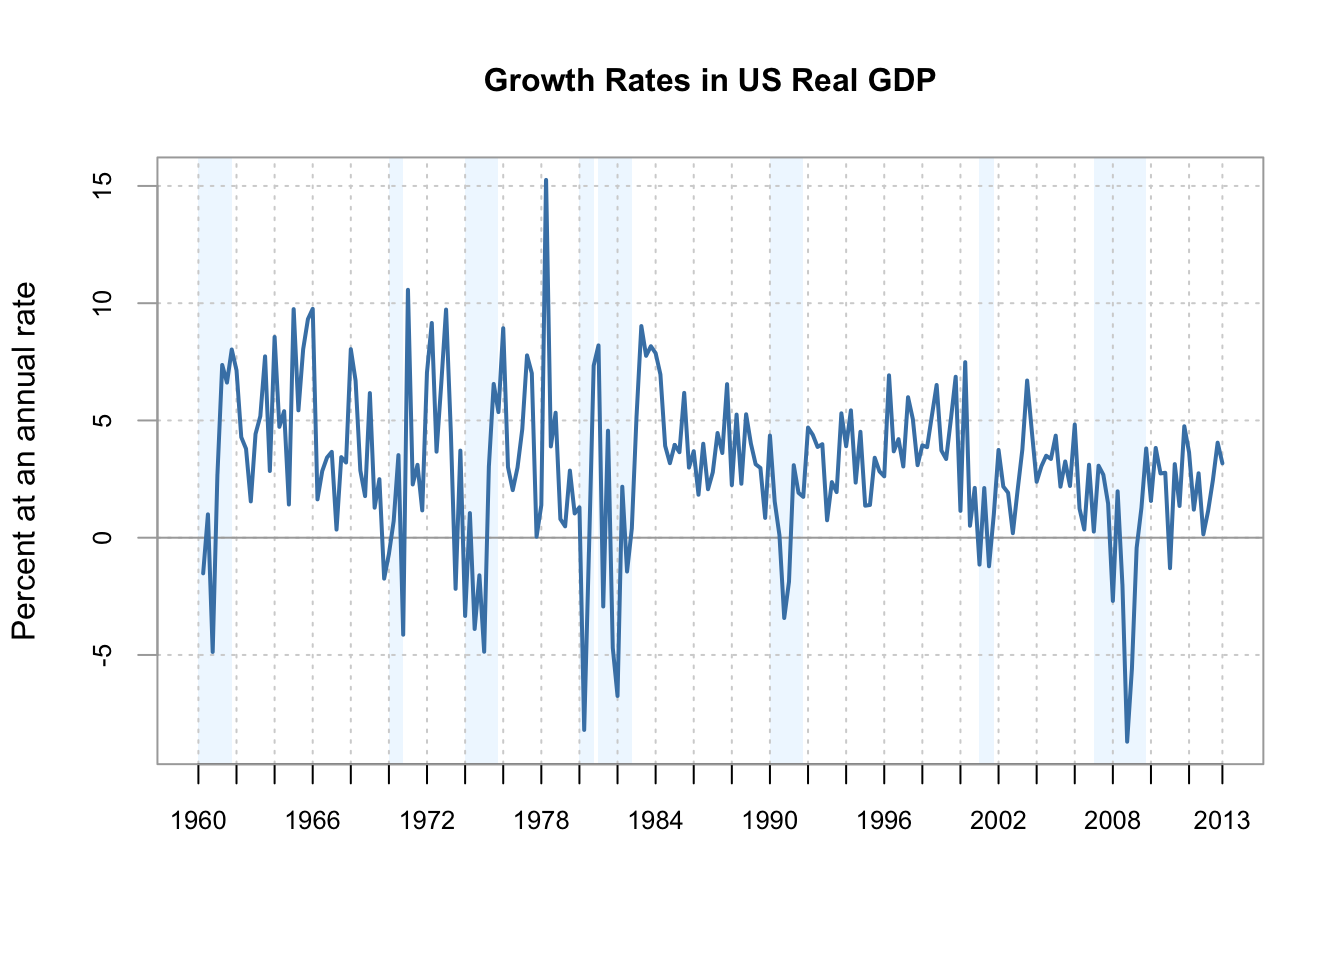
\includegraphics{bookdown-demo_files/figure-latex/unnamed-chunk-8-1} \end{center}

The plot (figure 4.2 in the book) shows the scatterplot of all
observations. We see that the points are strongly scatterd and an
apparent relationship cannot be detected by looking at it. Yet it can be
assumed that both variables are negatively correlated, that is we expect
to observe lower test scores in bigger classes.

The function \texttt{cor} can be used to compute the correlation between
2 numerical vectors.

\begin{Shaded}
\begin{Highlighting}[]
\KeywordTok{cor}\NormalTok{(CASchools}\OperatorTok{$}\NormalTok{STR, CASchools}\OperatorTok{$}\NormalTok{score)}
\end{Highlighting}
\end{Shaded}

\begin{verbatim}
## [1] -0.2263627
\end{verbatim}

As the scatterplot already suggested the correlation is negative but
rather weak.

The task we are facing now is to find the regression line which fits
best to the data. Of course we could simply do graphical inspection,
some correlation analysis and then select the best fitting line by
eyeballing. This is unscientific and prone to subjective perception:
different students would draw different regression lines. On this
account, we are interested in techniques that are more sophisticated.

\section{The Ordinary Least Squares (OLS)
Estimator}\label{the-ordinary-least-squares-ols-estimator}

The OLS estimator chooses the regression coefficients such that the
estimated regression line is as close as possible to the observed data
points. Closeness is measured by the sum of the squared mistakes made in
predicting \(Y\) given \(X\). Let \(b_0\) and \(b_1\) be some estimators
of \(\beta_0\) and \(\beta_1\). Then the sum of squared estimation
mistakes can be expressed as

\[ \sum^n_{i = 1} (Y_i - b_0 - b_1 X_i)^2. \]

The OLS estimator in the simple regression model is the pair of
estimators for intercept and slope which minimizes the expression above.
The dervivation of the OLS estimators for both parameters are presented
in Appendix 4.1 of the book. The results are summarized in Key Concept
4.2.

Key Concept 4.2

The OLS Estimator, Predicted Values, and Residuals

The OLS estimators of the slope \(\beta_1\) and the intercept
\(\beta_0\) in the simple linear regression model are

\begin{align}
  \hat{\beta}_1 & = \frac{ \sum_{i = 1}^n (X_i - \bar{X})(Y_i - \bar{Y}) } { \sum_{i=1}^n (X_i -   \bar{X})^2}  \\
  \\
  \hat{\beta}_0 & =  \bar{Y} - \hat{\beta}_1 \bar{X} 
\end{align}

The OLS predicted values \(\hat{Y}_i\) and residuals \(\hat{u}_i\) are

\begin{align}
  \hat{Y}_i & =  \hat{\beta}_0 + \hat{\beta}_1 X_i,\\
  \\
  \hat{u}_i & =  Y_i - \hat{Y}_i. 
\end{align}

The estimated intercept \((\hat{\beta}_0)\), the slope parameter
\((\hat{\beta}_1)\), and the residuals \(\left(\hat{u}_i\right)\) are
computed from a sample of \(n\) observations of \(X_i\) and \(Y_i\),
\(i\), \(...\), \(n\). These are \emph{estimates} of the unkown true
population intercept \(\left(\beta_0 \right)\), slope
\(\left(\beta_1\right)\), and error term \((u_i)\).

There are many possible ways to compute \(\left(\hat{\beta_0}\right)\)
and \(\left(\hat{\beta_1}\right)\) in R. We could implement the formulas
with two of R's most basic functions: \texttt{mean} and \texttt{sum}. Of
course there are also other and even more manual ways to do the same
tasks.

\begin{Shaded}
\begin{Highlighting}[]
\KeywordTok{attach}\NormalTok{(CASchools) }\CommentTok{#allows to use the variables contained in CASchools directly}
\end{Highlighting}
\end{Shaded}

\begin{verbatim}
## The following objects are masked from CASchools (pos = 3):
## 
##     calworks, computer, county, district, english, expenditure,
##     grades, income, lunch, math, read, school, score, STR,
##     students, teachers
\end{verbatim}

\begin{Shaded}
\begin{Highlighting}[]
\CommentTok{# compute beta_1 }
\NormalTok{beta_}\DecValTok{1}\NormalTok{ <-}\StringTok{ }\KeywordTok{sum}\NormalTok{((STR }\OperatorTok{-}\StringTok{ }\KeywordTok{mean}\NormalTok{(STR))}\OperatorTok{*}\NormalTok{(score }\OperatorTok{-}\StringTok{ }\KeywordTok{mean}\NormalTok{(score))) }\OperatorTok{/}\StringTok{ }\KeywordTok{sum}\NormalTok{((STR }\OperatorTok{-}\StringTok{ }\KeywordTok{mean}\NormalTok{(STR))}\OperatorTok{^}\DecValTok{2}\NormalTok{)}

\CommentTok{# compute beta_0}
\NormalTok{beta_}\DecValTok{0}\NormalTok{ <-}\StringTok{ }\KeywordTok{mean}\NormalTok{(score) }\OperatorTok{-}\StringTok{ }\NormalTok{beta_}\DecValTok{1} \OperatorTok{*}\StringTok{ }\KeywordTok{mean}\NormalTok{(STR)}

\CommentTok{# print the results to the console}
\NormalTok{beta_}\DecValTok{1}
\end{Highlighting}
\end{Shaded}

\begin{verbatim}
## [1] -2.279808
\end{verbatim}

\begin{Shaded}
\begin{Highlighting}[]
\NormalTok{beta_}\DecValTok{0}
\end{Highlighting}
\end{Shaded}

\begin{verbatim}
## [1] 698.9329
\end{verbatim}

OLS is one of the most widly-used estimation techniques. Being a
statistical programming language, R already contains a built-in function
named \texttt{lm} (\textbf{l}inear \textbf{m}odel) which can be used to
carry out regression analysis. The first argument of the function is the
regression formula with the basic syntax
\texttt{y\ \textasciitilde{}\ x} where \texttt{y} is the dependent
variable and \texttt{x} the explanatory variable. The argument
\texttt{data} specifies the data set to be used in the regression. We
now revisit the example from the book where the relationship between the
students' test scores and the class sizes is analysed. The following
code uses \texttt{lm} to replicate the results presented in figure 4.3
in the book.

\begin{Shaded}
\begin{Highlighting}[]
\CommentTok{# estimate the model and assign the result to linear_model}
\NormalTok{linear_model <-}\StringTok{ }\KeywordTok{lm}\NormalTok{(score }\OperatorTok{~}\StringTok{ }\NormalTok{STR, }\DataTypeTok{data =}\NormalTok{ CASchools)}

\CommentTok{# Print the standard output of the estimated lm object to the console }
\NormalTok{linear_model}
\end{Highlighting}
\end{Shaded}

\begin{verbatim}
## 
## Call:
## lm(formula = score ~ STR, data = CASchools)
## 
## Coefficients:
## (Intercept)          STR  
##      698.93        -2.28
\end{verbatim}

\begin{Shaded}
\begin{Highlighting}[]
\CommentTok{# plot the data}
\KeywordTok{plot}\NormalTok{(score }\OperatorTok{~}\StringTok{ }\NormalTok{STR, }
     \DataTypeTok{data =}\NormalTok{ CASchools,}
     \DataTypeTok{main =} \StringTok{"Scatterplot of Test Score vs. Class Size"}\NormalTok{, }
     \DataTypeTok{xlab =} \StringTok{"STR (X)"}\NormalTok{,}
     \DataTypeTok{ylab =} \StringTok{"Test Score (Y)"}\NormalTok{,}
     \DataTypeTok{xlim =} \KeywordTok{c}\NormalTok{(}\DecValTok{10}\NormalTok{, }\DecValTok{30}\NormalTok{),}
     \DataTypeTok{ylim =} \KeywordTok{c}\NormalTok{(}\DecValTok{600}\NormalTok{, }\DecValTok{720}\NormalTok{)}
\NormalTok{     )}

\CommentTok{# add the regression line}
\KeywordTok{abline}\NormalTok{(linear_model) }
\end{Highlighting}
\end{Shaded}

\begin{center}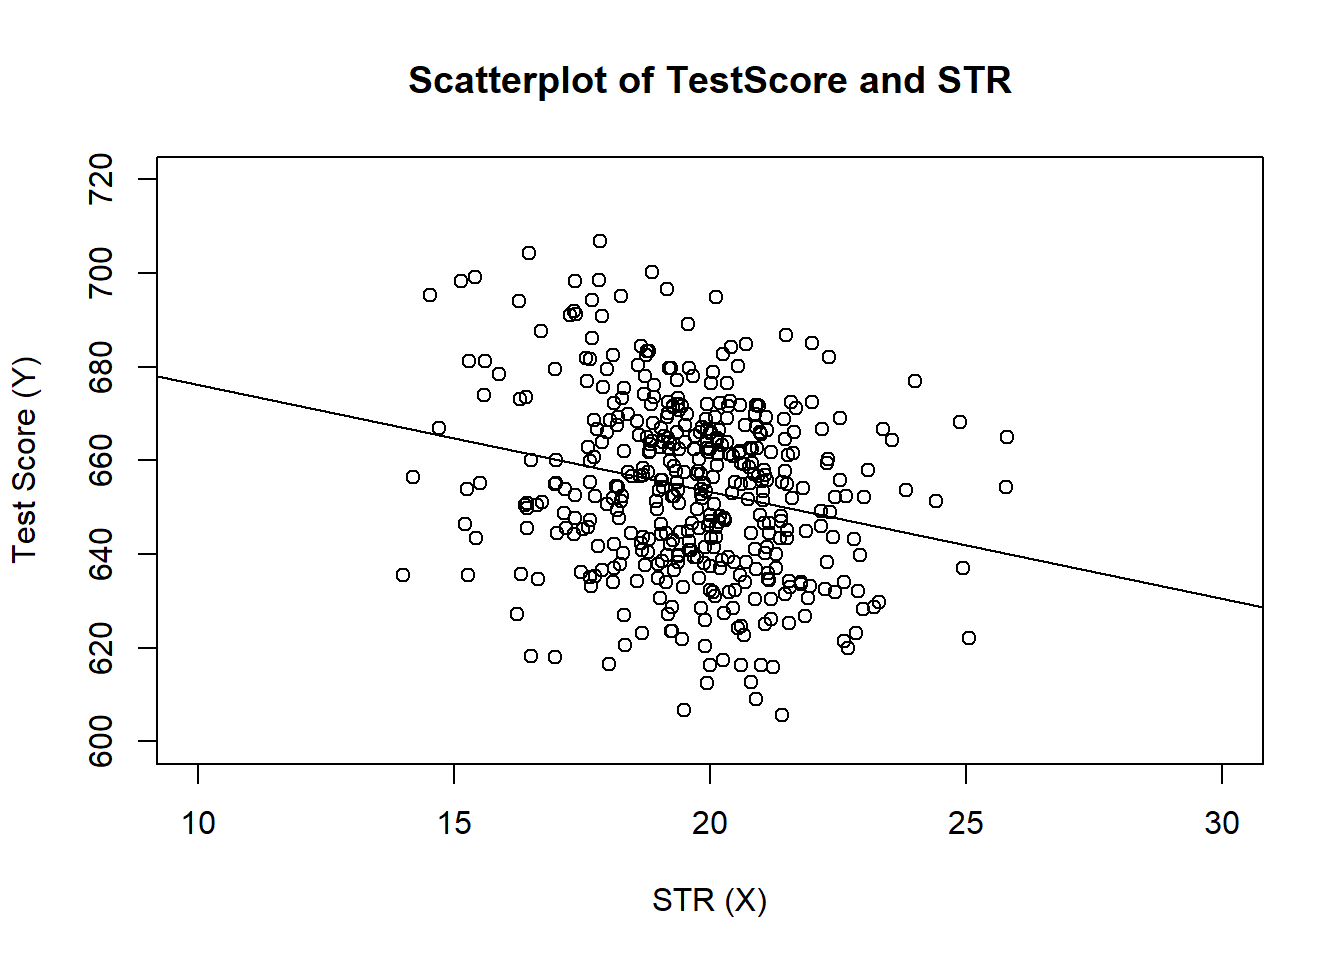
\includegraphics{bookdown-demo_files/figure-latex/unnamed-chunk-12-1} \end{center}

Did you notice that this time, we did not pass the intercept and slope
parameters to \texttt{abline}? If you call \texttt{abline} on an object
of class \texttt{lm} that only contains a single regressor variable,
Rdraws the regression line automatically!

\section{Measures of fit}\label{measures-of-fit}

After estimating a linear regression, the question occurs how well that
regression line describes the data. Are the observations tightly
clustered arround the regression line, or are they spread out? Both, the
\(R^2\) and the \emph{standard error of the regression} (\(SER\))
measure how well the OLS Regression line fits the data.

\subsection{\texorpdfstring{The \(R^2\)}{The R\^{}2}}\label{the-r2}

The \(R^2\) is the fraction of sample variance of \(Y_i\) that is
explained by \(X_i\). Mathemethically, the \(R^2\) can be written as the
ratio of the explained sum of squares to the total sum of squares. The
\emph{explained sum of squares} (\(ESS\)) is the sum of squared
deviations of the predicted values, \(\hat{Y_i}\), from the average of
the \(Y_i\). The \emph{total sum of squares} (\(TSS\)) is the sum of
squared deviations of the \(Y_i\) from their average.

\begin{align}
  ESS & =  \sum_{i = 1}^n \left( \hat{Y_i} - \bar{Y} \right)^2   \\
  \\
  TSS & =  \sum_{i = 1}^n \left( Y_i - \bar{Y} \right)^2   \\
  \\
  R^2 & = \frac{ESS}{TSS}
\end{align}

Since \(TSS = ESS + SSR\) we can also write

\[ R^2 = 1- \frac{SSR}{TSS} \]

where \(SSR\) is the sum of squared residuals, a measure for the errors
made when predicting the \(Y\) by \(X\). The SSR is defined as

\[ SSR = \sum_{i=1}^n \hat{u}_i^2. \]

\(R^2\) lies between \(0\) and \(1\). It is easy to see that a perfect
fit, i.e.~no errors made when fitting the regression line, implies
\(R^2 = 1\) since then we have \(SSR=0\). On the contrary, if our
estimated regression line does not explain any variation in the \(Y_i\),
we have \(ESS=0\) and consequently \(R^2=0\).

\subsection{Standard Error of the
Regression}\label{standard-error-of-the-regression}

The \emph{Standard Error of the Regression} (\(SER\)) is an estimator of
the standard deviation of the regression error \(\hat{u}_i\). As such it
measure the magnitude of a typical deviation from the regression,
i.e.~the magnitude of a typical regression error.

\[ SER = s_{\hat{u}} = \sqrt{s_{\hat{u}}^2} \ \ \ \text{where} \ \ \ s_{\hat{u} }^2 = \frac{1}{n-2} \sum_{i = 1}^n \hat{u}^2_i = \frac{SSR}{n - 2} \]

Remember that the \(u_i\) are unobserved. That is why we use their
estimated counterparts, the residuals \(\hat{u}_i\) instead. See chapter
4.3 of the book for a more detailed comment on the \(SER\).

\subsection{Application to the Test Score
Data}\label{application-to-the-test-score-data}

Both measures of fit can be obtained by using the function
\texttt{summary} with the \texttt{lm} object provided as the only
argument. Whereas \texttt{lm} only prints out the coefficients,
\texttt{summary} provides additional predefined information such as the
\(R^2\) and the \(SER\).

\begin{Shaded}
\begin{Highlighting}[]
\NormalTok{mod_summary <-}\StringTok{ }\KeywordTok{summary}\NormalTok{(linear_model)}
\NormalTok{mod_summary}
\end{Highlighting}
\end{Shaded}

\begin{verbatim}
## 
## Call:
## lm(formula = score ~ STR, data = CASchools)
## 
## Residuals:
##     Min      1Q  Median      3Q     Max 
## -47.727 -14.251   0.483  12.822  48.540 
## 
## Coefficients:
##             Estimate Std. Error t value Pr(>|t|)    
## (Intercept) 698.9329     9.4675  73.825  < 2e-16 ***
## STR          -2.2798     0.4798  -4.751 2.78e-06 ***
## ---
## Signif. codes:  0 '***' 0.001 '**' 0.01 '*' 0.05 '.' 0.1 ' ' 1
## 
## Residual standard error: 18.58 on 418 degrees of freedom
## Multiple R-squared:  0.05124,    Adjusted R-squared:  0.04897 
## F-statistic: 22.58 on 1 and 418 DF,  p-value: 2.783e-06
\end{verbatim}

The \(R^2\) in the output is called `Multiple R-squared' and takes the
value \(0.051\). Hence, \(5.1 \%\) of the variance of the dependent
variable \(score\) is explained by the explanatory variable \(STR\).
That is the regression explains some of the variance but much of the
variation in test scores remains unexplained (compare figure 4.3 in the
book).

The \(SER\) is called `Residual standard error' and takes the value
\(18.58\). The unit of the \(SER\) is the same as the unit of the
dependent variable. In out context we can interpret the value as
follows: on average the deviation of the actual achieved test score and
the regression line is \(18.58\) points.

Now, let us check whether the \texttt{summary} function uses the same
definition for \(R^2\) and \(SER\) as we do by computing them manually.

\begin{Shaded}
\begin{Highlighting}[]
\CommentTok{# compute R^2 manually}
\NormalTok{SSR <-}\StringTok{ }\KeywordTok{sum}\NormalTok{(mod_summary}\OperatorTok{$}\NormalTok{residuals}\OperatorTok{^}\DecValTok{2}\NormalTok{)}
\NormalTok{TSS <-}\StringTok{ }\KeywordTok{sum}\NormalTok{((score }\OperatorTok{-}\StringTok{ }\KeywordTok{mean}\NormalTok{(score))}\OperatorTok{^}\DecValTok{2}\NormalTok{)}
\NormalTok{R2 <-}\StringTok{ }\DecValTok{1} \OperatorTok{-}\StringTok{ }\NormalTok{SSR}\OperatorTok{/}\NormalTok{TSS}
\NormalTok{R2}
\end{Highlighting}
\end{Shaded}

\begin{verbatim}
## [1] 0.05124009
\end{verbatim}

\begin{Shaded}
\begin{Highlighting}[]
\CommentTok{# compute SER manually}
\NormalTok{n <-}\StringTok{ }\KeywordTok{nrow}\NormalTok{(CASchools)}
\NormalTok{SER <-}\StringTok{ }\KeywordTok{sqrt}\NormalTok{(SSR }\OperatorTok{/}\StringTok{ }\NormalTok{(n}\OperatorTok{-}\DecValTok{2}\NormalTok{))}
\NormalTok{SER}
\end{Highlighting}
\end{Shaded}

\begin{verbatim}
## [1] 18.58097
\end{verbatim}

We find that the results coincide.

\section{The Least Squares
Assumptions}\label{the-least-squares-assumptions}

OLS performs well under a great variety of different circumstances.
However, there are some assumptions which are posed on the data which
need to be satisfied in order to achieve reliable results.

Key Concept 4.3

The Least Squares Assumptions

\[Y_i = \beta_0 + \beta_1 X_i + u_i \text{, } i = 1, ...,n \text{, where} \]

\begin{enumerate}
\def\labelenumi{\arabic{enumi}.}
\tightlist
\item
  The error term \(u_i\) has conditional mean zero given \(X_i\):
  \(E(u_i|X_i) = 0\)
\item
  \((X_i,Y_i), i = 1,...,n\) are independent and identically distributed
  (i.i.d.) draws from their joint distribution
\item
  Large outliers are unlikely: \(X_i\) and \(Y_i\) have nonzero finite
  fourth moments
\end{enumerate}

\subsection{Assumption \#1: The Error Term has Conditional Mean of
Zero}\label{assumption-1-the-error-term-has-conditional-mean-of-zero}

This means that no matter which \(X\)-value we choose, the error term
should not show any systematic pattern and have a mean of \(0\).
Consider the case that \(E(u) = 0\) but for low and high values of
\(X\), the error term tends to be positive and for midrange values of
\(X\) the error tends to be negative. We can use R to construct such an
example. To do so we generate our own data using R's build in random
number generators. We can start by creating a vector of \(X\)-values.
For our example we decide to generate uniformly distributed numbers
which can be done with the function \texttt{runif}. We also need to
simulate the error term. For this we generate normally distributed
numbers with a mean equal to \(0\). Finally, the \(Y\)-value is obtained
as a quadratic function of the \(X\)-values and the error term. Next, we
plot the simulated data and add a the estimated regression line of a
simple regression model as well as the predictions made with a quadratic
model.

\begin{Shaded}
\begin{Highlighting}[]
\CommentTok{# set a random seed to make the results reproducible}
\KeywordTok{set.seed}\NormalTok{(}\DecValTok{321}\NormalTok{)}

\CommentTok{# simulate the data }
\NormalTok{X <-}\StringTok{ }\KeywordTok{runif}\NormalTok{(}\DecValTok{50}\NormalTok{, }\DataTypeTok{min =} \OperatorTok{-}\DecValTok{5}\NormalTok{, }\DataTypeTok{max =} \DecValTok{5}\NormalTok{)}
\NormalTok{u <-}\StringTok{ }\KeywordTok{rnorm}\NormalTok{(}\DecValTok{50}\NormalTok{, }\DataTypeTok{sd =} \DecValTok{5}\NormalTok{)             }
\NormalTok{Y <-}\StringTok{ }\NormalTok{X}\OperatorTok{^}\DecValTok{2} \OperatorTok{+}\StringTok{ }\DecValTok{2}\OperatorTok{*}\NormalTok{X }\OperatorTok{+}\StringTok{ }\NormalTok{u }\CommentTok{# the true relation                  }

\CommentTok{# estimate a simple regression model }
\NormalTok{mod_simple <-}\StringTok{ }\KeywordTok{lm}\NormalTok{(Y }\OperatorTok{~}\StringTok{ }\NormalTok{X)}

\CommentTok{# precit using a quadratic model }
\NormalTok{prediction <-}\StringTok{ }\KeywordTok{predict}\NormalTok{(}\KeywordTok{lm}\NormalTok{(Y }\OperatorTok{~}\StringTok{ }\NormalTok{X }\OperatorTok{+}\StringTok{  }\KeywordTok{I}\NormalTok{(X}\OperatorTok{^}\DecValTok{2}\NormalTok{)), }\KeywordTok{data.frame}\NormalTok{(}\DataTypeTok{X =} \KeywordTok{sort}\NormalTok{(X)))}

\CommentTok{# plot the results}
\KeywordTok{plot}\NormalTok{(Y }\OperatorTok{~}\StringTok{ }\NormalTok{X)}
\KeywordTok{abline}\NormalTok{(mod_simple, }\DataTypeTok{col =} \StringTok{"red"}\NormalTok{)}
\KeywordTok{lines}\NormalTok{(}\KeywordTok{sort}\NormalTok{(X), prediction)}
\end{Highlighting}
\end{Shaded}

\begin{center}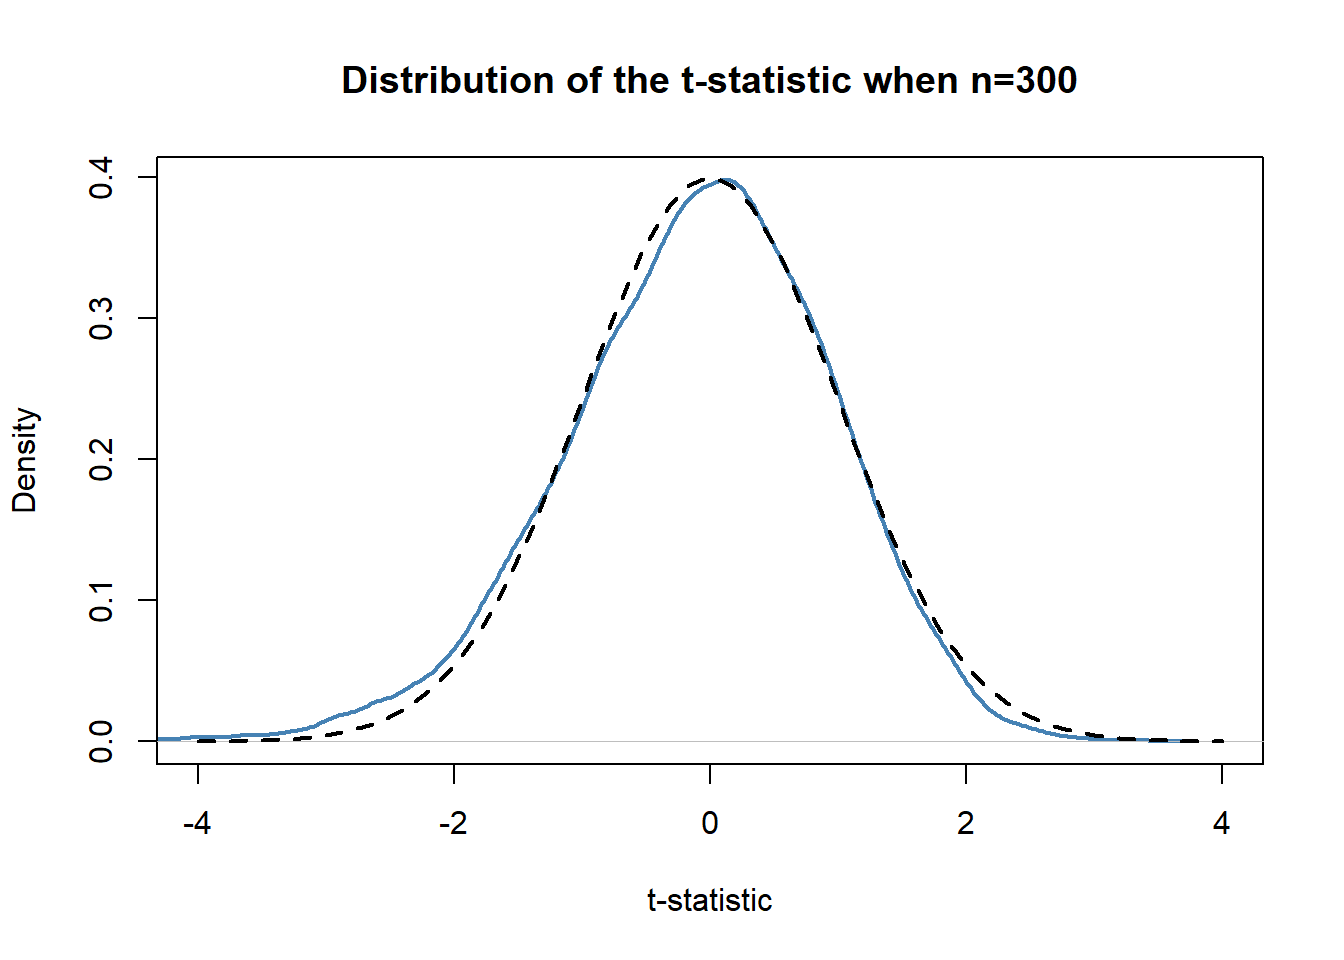
\includegraphics{bookdown-demo_files/figure-latex/unnamed-chunk-15-1} \end{center}

This shows what is meant by \(E(u_i|X_i) = 0\): using the quadratic
model we see that there are no systematic deviations of the observation
from the predicted relation. It is credible that the assumption is not
violated when such a model is employed. However, using a simple linear
regression model we see that the assumption is probably violated as
\(E(u_i|X_i)\) varies with the \(X_i\).

\subsection{\texorpdfstring{Assumption \#2: All \((X_i, Y_i)\) are
Independtly and Identically
Distributed}{Assumption \#2: All (X\_i, Y\_i) are Independtly and Identically Distributed}}\label{assumption-2-all-x_i-y_i-are-independtly-and-identically-distributed}

Most common sampling schemes used when collecting data from populations
produce i.i.d. samples. For example, we could use R's random number
generator to randomly select student IDs from a university's enrollment
list and record age \(X\) and earnings \(Y\) of the corresponding
students. This is a typical example of simple random sampling and
ensures that all the \(X_i,Y_i\) are drawn randomly from the same
population.

A prominent example where the i.i.d. assumption is not fulfilled is time
series data where we have observations on the same unit over time. For
example, take \(X\) as the number of workers employed by a production
company over the course of time. Due to technological change, the
company makes job cuts time after time. Using R we can simulate such a
process and plot it. We start the series with a total of 5000 workers
and simulate the reduction of employment as a declining process with
normal distributed random influences.

\begin{Shaded}
\begin{Highlighting}[]
\CommentTok{# set random seed}
\KeywordTok{set.seed}\NormalTok{(}\DecValTok{7}\NormalTok{)}

\CommentTok{# initialize the employment vector}
\NormalTok{X <-}\StringTok{ }\KeywordTok{c}\NormalTok{(}\DecValTok{5000}\NormalTok{,}\KeywordTok{rep}\NormalTok{(}\OtherTok{NA}\NormalTok{,}\DecValTok{99}\NormalTok{))}

\CommentTok{# generate a date vector}
\NormalTok{Date <-}\StringTok{ }\KeywordTok{seq}\NormalTok{(}\KeywordTok{as.Date}\NormalTok{(}\StringTok{"1951/1/1"}\NormalTok{), }\KeywordTok{as.Date}\NormalTok{(}\StringTok{"2050/1/1"}\NormalTok{), }\StringTok{"years"}\NormalTok{)}

\CommentTok{# generate time series observations with random influences}
\ControlFlowTok{for}\NormalTok{ (i }\ControlFlowTok{in} \DecValTok{2}\OperatorTok{:}\DecValTok{100}\NormalTok{) X[i] <-}\StringTok{ }\FloatTok{0.98}\OperatorTok{*}\NormalTok{X[i}\OperatorTok{-}\DecValTok{1}\NormalTok{] }\OperatorTok{+}\StringTok{ }\KeywordTok{rnorm}\NormalTok{(}\DecValTok{1}\NormalTok{, }\DataTypeTok{sd=}\DecValTok{200}\NormalTok{)}

\CommentTok{#plot the results}
\KeywordTok{plot}\NormalTok{(Date, X, }\DataTypeTok{type =} \StringTok{"l"}\NormalTok{, }\DataTypeTok{col=}\StringTok{"steelblue"}\NormalTok{, }\DataTypeTok{ylab =} \StringTok{"Workers"}\NormalTok{)}
\end{Highlighting}
\end{Shaded}

\begin{center}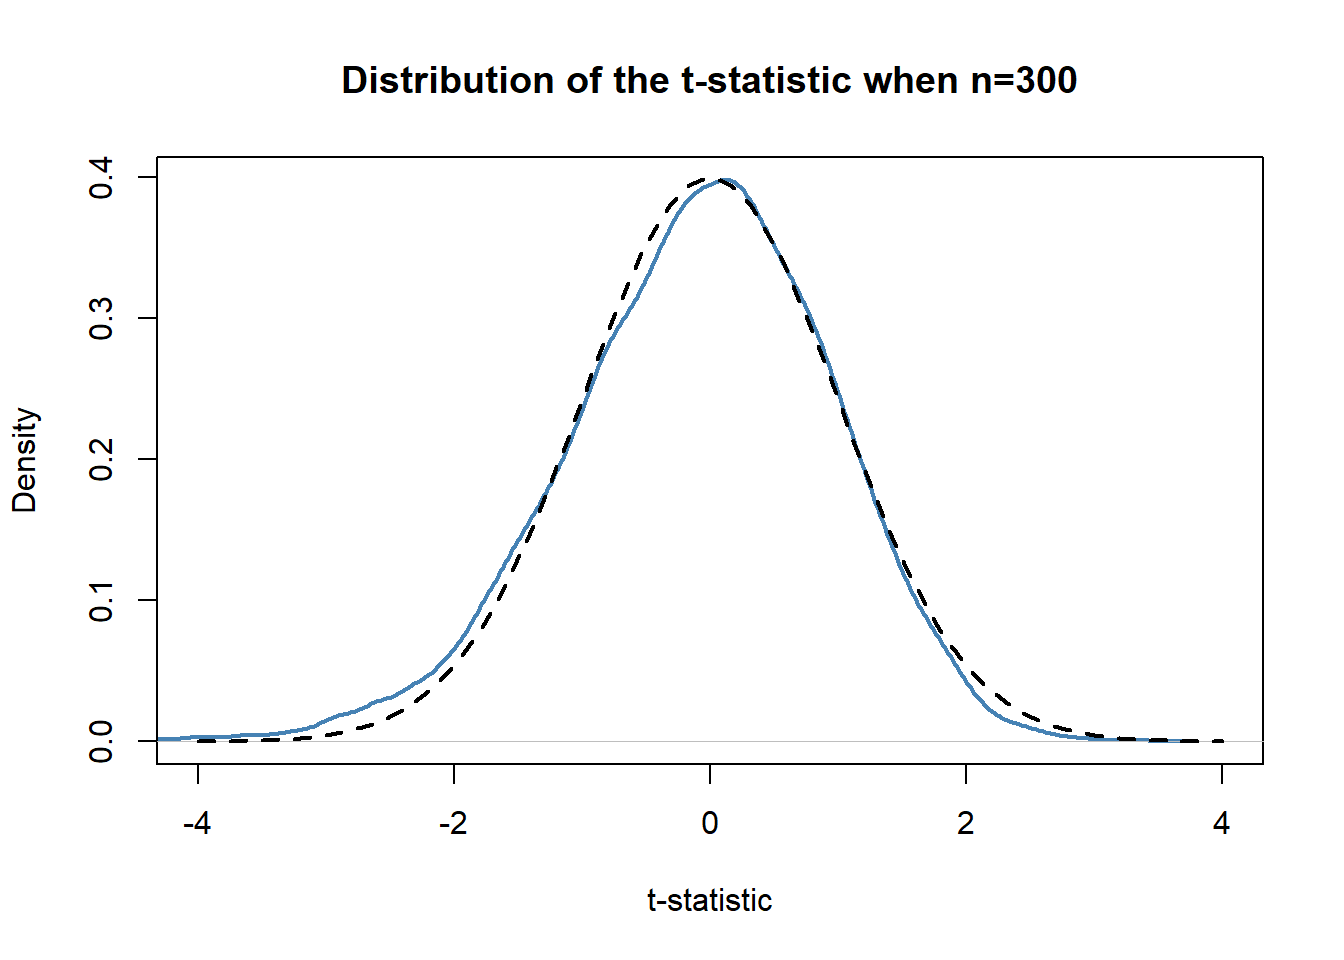
\includegraphics{bookdown-demo_files/figure-latex/unnamed-chunk-16-1} \end{center}

It is evident that the observations on \(X\) cannot be independnet in
this example: the level of today's employment is correlated with
tomorrows employment level. Thus, the i.i.d. assumption is violated for
\(X\).

\subsection{Assumption \#3: Sensitivity to
Outliers}\label{assumption-3-sensitivity-to-outliers}

\begin{Shaded}
\begin{Highlighting}[]
\KeywordTok{set.seed}\NormalTok{(}\DecValTok{123}\NormalTok{)}
\NormalTok{x     <-}\StringTok{ }\KeywordTok{sort}\NormalTok{(}\KeywordTok{runif}\NormalTok{(}\DecValTok{10}\NormalTok{, }\DataTypeTok{min =} \DecValTok{30}\NormalTok{, }\DataTypeTok{max =} \DecValTok{70}\NormalTok{ ))}
\NormalTok{y     <-}\StringTok{ }\KeywordTok{rnorm}\NormalTok{(}\DecValTok{10}\NormalTok{ , }\DataTypeTok{mean =} \DecValTok{200}\NormalTok{, }\DataTypeTok{sd =} \DecValTok{50}\NormalTok{)}
\NormalTok{y[}\DecValTok{9}\NormalTok{] <-}\StringTok{ }\DecValTok{2000}

\NormalTok{fit               <-}\StringTok{ }\KeywordTok{lm}\NormalTok{(y }\OperatorTok{~}\StringTok{ }\NormalTok{x)}
\NormalTok{fitWithoutOutlier <-}\StringTok{ }\KeywordTok{lm}\NormalTok{(y[}\OperatorTok{-}\DecValTok{9}\NormalTok{] }\OperatorTok{~}\StringTok{ }\NormalTok{x[}\OperatorTok{-}\DecValTok{9}\NormalTok{])}

\KeywordTok{plot}\NormalTok{(y }\OperatorTok{~}\StringTok{ }\NormalTok{x)}
\KeywordTok{abline}\NormalTok{(fit)}
\KeywordTok{abline}\NormalTok{(fitWithoutOutlier, }\DataTypeTok{col =} \StringTok{"red"}\NormalTok{)}
\end{Highlighting}
\end{Shaded}

\begin{center}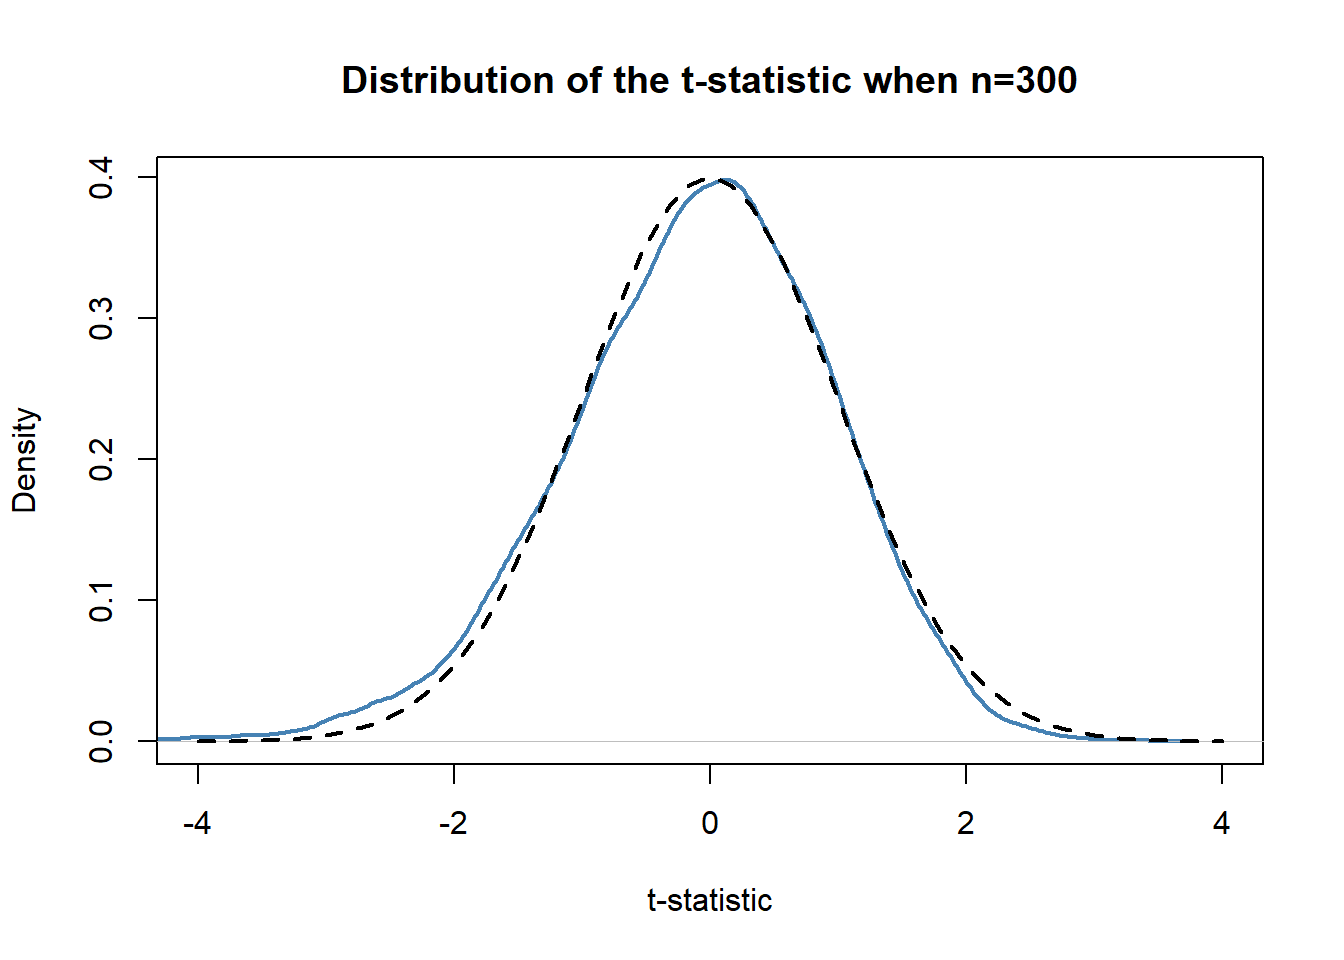
\includegraphics{bookdown-demo_files/figure-latex/unnamed-chunk-17-1} \end{center}

\hypertarget{vizslrm}{}

\section{The Sampling Distribution of the OLS
Estimator}\label{the-sampling-distribution-of-the-ols-estimator}

Because the OLS estimators \(\hat{\beta_0}\) and \(\hat{\beta_1}\) are
computed from a randomly drawn sample, the estimators themselves are
random variables with a probability distribution --- the sampling
distribution --- that describes the values they could take over
different random samples. Although the sampling distribution of
\(\hat{\beta_0}\) and \(\hat{\beta_1}\) can be complicated when the
sample size is small, it is possible to make certain statements about it
that hold for all \(n\). In particular
\[ E(\hat{\beta_0}) = \beta_0 \ \ \text{and} \ \  E(\hat{\beta_1}) = \beta_1,\]
that is, \(\hat{\beta_0}\) and \(\hat{\beta_1}\) are unbiased estimators
of \(\beta_0\) and \(\beta_1\). If the sample is sufficiently large, by
the central limit theorem the sampling distribution of the estimators is
well approximated by the bivariate normal distribution (2.1). This
implies that the marginal distributions are also normal in large
samples. Core facts of the large-sample distribution of \(\beta_0\) and
\(\beta_1\) are presented in Key Concept 4.4.

Key Concept 4.4

Large Sample Distribution of \(\hat{\beta_0}\) and \(\hat{\beta_1}\)

If the least squares assumptions in Key Concept 4.3 hold, then in
large-samples \(\hat{\beta_0}\) and \(\hat{\beta_1}\) have a jointly
normal sampling distribution. The large sample normal distribution of
\(\hat{\beta_1}\) is \(N(\beta_1, \sigma^2_\hat{\beta_1})\), where the
variance of the distribution, \(\sigma^2_\hat{\beta_1}\), is

\[ \sigma^2_\hat{\beta_1} = \frac{1}{n} \frac{Var \left[ \left(X_i - \mu_X \right) u_i  \right]}  {\left[  Var \left(X_i \right)  \right]^2} \tag{4.1} \]

The large sample normal distribution of \(\hat{\beta_0}\) is
\(N(\beta_0, \sigma^2_\hat{\beta_0})\), where

\[ \sigma^2_\hat{\beta_0} =  \frac{1}{n} \frac{Var \left( H_i u_i \right)}{ \left[  E \left(H_i^2  \right)  \right]^2 } \ , \ \text{where} \ \ H_i = 1 - \left[ \frac{\mu_X} {E \left( X_i^2\right)} \right] X_i. \tag{4.2} \]

Whether this really holds can be verified using R. First we build our
own population of \(100000\) observations in total. To do this we need
values for our independent variable \(X\), for the error term \(u\), and
the regression parameters \(\beta_0\) and \(\beta_1\). With all this
combined in a simple regression model, we can compute our dependent
variable \(Y\). In our example we generate the numbers \(X_i\),
\(i = 1\), \ldots{} ,\(100000\) by drawing a random sample from a
uniform distribution on the interval \([0,20]\). The realisations of the
error terms \(u_i\) are drawn from a standard normal distribution with
parameters \(\mu = 0\) and \(\sigma^2 = 100\) (note that \texttt{rnorm}
requires \(\sigma\) as input for the argument \texttt{sd}). Furthermore
we chose \(\beta_0 = -2\) and \(\beta_1 = 3.5\). Finally, we store the
result in a dataframe.

\begin{Shaded}
\begin{Highlighting}[]
\CommentTok{# simulate data}
\NormalTok{N <-}\StringTok{ }\DecValTok{100000}
\NormalTok{X <-}\StringTok{ }\KeywordTok{runif}\NormalTok{(N, }\DataTypeTok{min =} \DecValTok{0}\NormalTok{, }\DataTypeTok{max =} \DecValTok{20}\NormalTok{)}
\NormalTok{u <-}\StringTok{ }\KeywordTok{rnorm}\NormalTok{(N, }\DataTypeTok{sd =} \DecValTok{10}\NormalTok{)}

\CommentTok{# population regression}
\NormalTok{Y <-}\StringTok{ }\OperatorTok{-}\DecValTok{2} \OperatorTok{+}\StringTok{ }\FloatTok{3.5}\OperatorTok{*}\NormalTok{X }\OperatorTok{+}\StringTok{ }\NormalTok{u}
\NormalTok{population <-}\StringTok{ }\KeywordTok{data.frame}\NormalTok{(X, Y)}
\end{Highlighting}
\end{Shaded}

From now on we will consider the previously generated data as the truth
(which of course would be \emph{unknown} in a real world application).
This knowledge about the true relationship between \(Y\) and \(X\) can
be used to verify the statements of key concept 4.4.

First, let us calculate the variances \(\sigma^2_\hat{\beta_0}\) and
\(\sigma^2_\hat{\beta_1}\) for a given sample size \(n = 100\).

\begin{Shaded}
\begin{Highlighting}[]
\CommentTok{# set sample size}
\NormalTok{n <-}\StringTok{ }\DecValTok{100}

\CommentTok{# compute the variance of hat_beta_1}
\NormalTok{var_b1 <-}\StringTok{ }\KeywordTok{var}\NormalTok{( ( X }\OperatorTok{-}\StringTok{ }\KeywordTok{mean}\NormalTok{(X) ) }\OperatorTok{*}\StringTok{ }\NormalTok{u ) }\OperatorTok{/}\StringTok{ }\NormalTok{(}\DecValTok{100} \OperatorTok{*}\StringTok{ }\KeywordTok{var}\NormalTok{(X)}\OperatorTok{^}\DecValTok{2}\NormalTok{)}

\CommentTok{# compute the variance of hat_beta_0}
\NormalTok{H_i <-}\StringTok{ }\DecValTok{1} \OperatorTok{-}\StringTok{ }\KeywordTok{mean}\NormalTok{(X) }\OperatorTok{/}\StringTok{ }\KeywordTok{mean}\NormalTok{(X}\OperatorTok{^}\DecValTok{2}\NormalTok{) }\OperatorTok{*}\StringTok{ }\NormalTok{X}
\NormalTok{var_b0 <-}\StringTok{ }\KeywordTok{var}\NormalTok{(H_i }\OperatorTok{*}\StringTok{ }\NormalTok{u) }\OperatorTok{/}\StringTok{ }\NormalTok{(n }\OperatorTok{*}\StringTok{ }\KeywordTok{mean}\NormalTok{(H_i}\OperatorTok{^}\DecValTok{2}\NormalTok{)}\OperatorTok{^}\DecValTok{2}\NormalTok{ )}
\end{Highlighting}
\end{Shaded}

\begin{Shaded}
\begin{Highlighting}[]
\CommentTok{# print variances to the console}
\NormalTok{var_b1}
\end{Highlighting}
\end{Shaded}

\begin{verbatim}
## [1] 0.03018694
\end{verbatim}

\begin{Shaded}
\begin{Highlighting}[]
\NormalTok{var_b0}
\end{Highlighting}
\end{Shaded}

\begin{verbatim}
## [1] 4.045066
\end{verbatim}

Now let us assume that we do not know the true values for \(\beta_0\)
and \(\beta_1\) and that it is not possible to observe the whole
population. However, we can observe a random sample of \(n\)
observations. Then, it would not be possible to compute the true
parameters but we could obtain estimates of \(\beta_0\) and \(\beta_1\)
from the sample data using OLS. However, we now that these estimates are
outcomes of random variables themselves since the observations are
randomly sampled from the population. Key Concept 4.4. describes their
distributions for large \(n\). When drawing a single sample of size
\(n\) it is not possible to make any statement about these
distributions. Things change if we repeat the sampling scheme many times
and compute the estimates for each sample: using such a procedure we
simulate outcomes of the respective distributions.

To achieve this in R, we employ the following approach:

\begin{itemize}
\tightlist
\item
  We assign the number of repetitions, \(500\) say, to \texttt{reps}.
  Then we initialize a matrix \texttt{fit} were the estimates obtained
  in each sampling iteration shall be stored row-wise. Thus \texttt{fit}
  has to be of dimensions \texttt{reps}\(\times2\).
\item
  In the next step we draw \texttt{reps} random sample of size
  \texttt{n} from the population and obtain OLS estimates for each
  sample. The results are stored as row entries in the outcome matrix
  \texttt{fit}. This is done using a \texttt{for} loop
\item
  At last, we estimate variances of both coefficient estimators using
  the sampled outcomes and plot histograms of the latter
\end{itemize}

\begin{Shaded}
\begin{Highlighting}[]
\CommentTok{# set repetions and sample size}
\NormalTok{n <-}\StringTok{ }\DecValTok{100}
\NormalTok{reps <-}\StringTok{ }\DecValTok{500}

\CommentTok{# initialize the matrix of outcomes}
\NormalTok{fit <-}\StringTok{ }\KeywordTok{matrix}\NormalTok{(}\DataTypeTok{ncol =} \DecValTok{2}\NormalTok{, }\DataTypeTok{nrow =}\NormalTok{ reps)}

\CommentTok{# loop sampling and estimating of the coefficients}
\ControlFlowTok{for}\NormalTok{ (i }\ControlFlowTok{in} \DecValTok{1}\OperatorTok{:}\NormalTok{reps)\{}
\NormalTok{ sample <-}\StringTok{ }\NormalTok{population[}\KeywordTok{sample}\NormalTok{(}\DecValTok{1}\OperatorTok{:}\NormalTok{N, n),]}
\NormalTok{ fit[i, ] <-}\StringTok{ }\KeywordTok{lm}\NormalTok{(Y }\OperatorTok{~}\StringTok{ }\NormalTok{X, }\DataTypeTok{data =}\NormalTok{ sample)}\OperatorTok{$}\NormalTok{coefficients}
\NormalTok{\}}

\CommentTok{# compute variance estimates using outcomes}
\KeywordTok{var}\NormalTok{(fit[ ,}\DecValTok{1}\NormalTok{])}
\end{Highlighting}
\end{Shaded}

\begin{verbatim}
## [1] 4.013954
\end{verbatim}

\begin{Shaded}
\begin{Highlighting}[]
\KeywordTok{var}\NormalTok{(fit[ ,}\DecValTok{2}\NormalTok{])}
\end{Highlighting}
\end{Shaded}

\begin{verbatim}
## [1] 0.02916391
\end{verbatim}

\begin{Shaded}
\begin{Highlighting}[]
\CommentTok{# plot histograms of beta_0 estimates}
\KeywordTok{hist}\NormalTok{(fit[ ,}\DecValTok{1}\NormalTok{], }\DataTypeTok{main =} \KeywordTok{bquote}\NormalTok{(The }\OperatorTok{~}\StringTok{ }\NormalTok{Distribution  }\OperatorTok{~}\StringTok{ }\NormalTok{of }\OperatorTok{~}\StringTok{ }\DecValTok{500} \OperatorTok{~}\StringTok{ }\NormalTok{beta[}\DecValTok{1}\NormalTok{] }\OperatorTok{~}\StringTok{ }\NormalTok{Estimates), }\DataTypeTok{xlab =} \KeywordTok{bquote}\NormalTok{(}\KeywordTok{hat}\NormalTok{(beta)[}\DecValTok{1}\NormalTok{]), }\DataTypeTok{freq =}\NormalTok{ F)}
\end{Highlighting}
\end{Shaded}

\begin{center}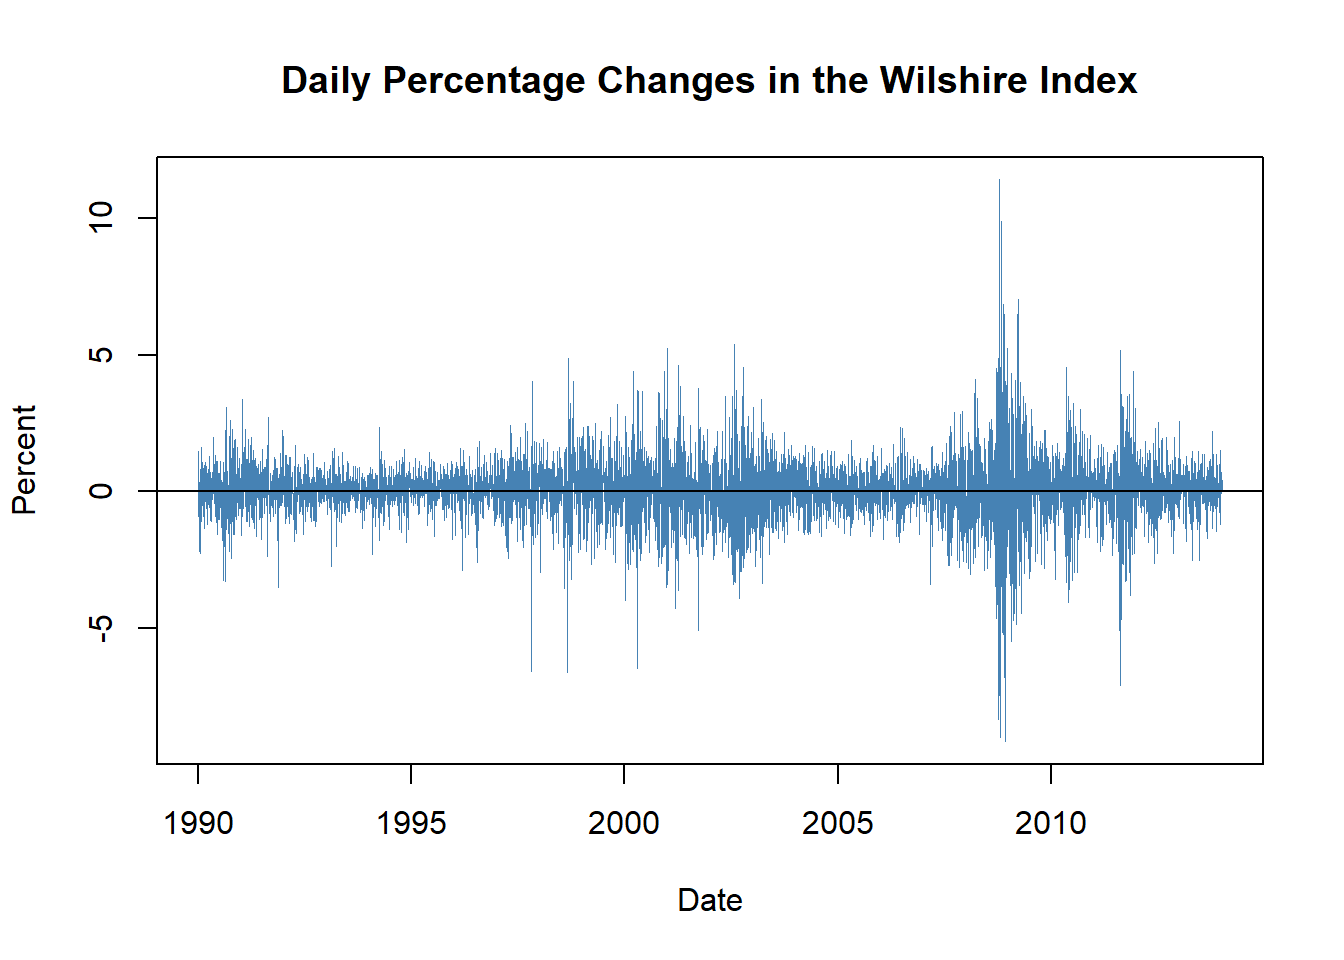
\includegraphics{bookdown-demo_files/figure-latex/unnamed-chunk-21-1} \end{center}

\begin{Shaded}
\begin{Highlighting}[]
\CommentTok{# plot histograms of beta_1 estimates}
\KeywordTok{hist}\NormalTok{(fit[ ,}\DecValTok{2}\NormalTok{], }\DataTypeTok{main =} \KeywordTok{bquote}\NormalTok{(The }\OperatorTok{~}\StringTok{ }\NormalTok{Distribution  }\OperatorTok{~}\StringTok{ }\NormalTok{of }\OperatorTok{~}\StringTok{ }\DecValTok{500} \OperatorTok{~}\StringTok{ }\NormalTok{beta[}\DecValTok{2}\NormalTok{] }\OperatorTok{~}\StringTok{ }\NormalTok{Estimates), }\DataTypeTok{xlab =} \KeywordTok{bquote}\NormalTok{(}\KeywordTok{hat}\NormalTok{(beta)[}\DecValTok{2}\NormalTok{]), }\DataTypeTok{freq =}\NormalTok{ F)}
\end{Highlighting}
\end{Shaded}

\begin{center}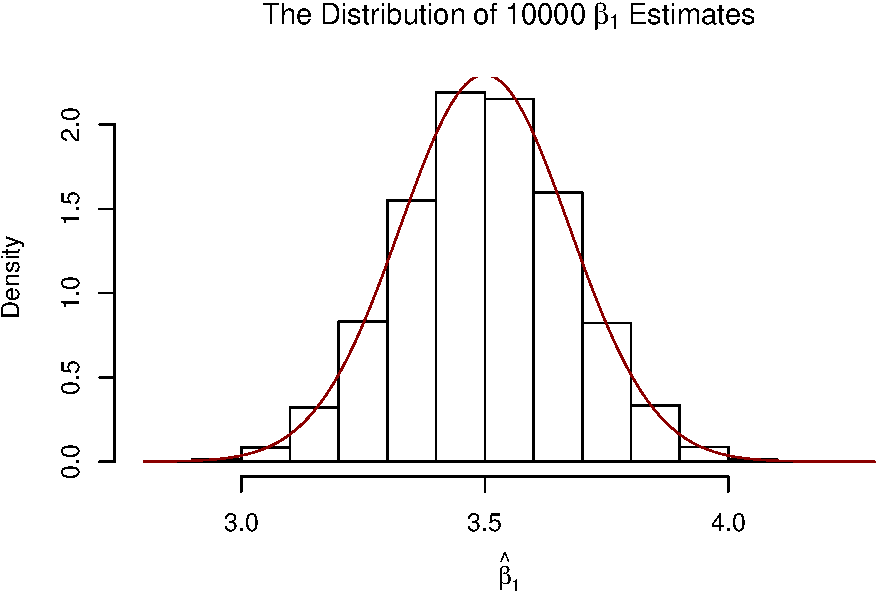
\includegraphics{bookdown-demo_files/figure-latex/unnamed-chunk-21-2} \end{center}

Now we are able to say the following with repspect to Key Concept 4.4:
first, our variance estimates are in favour of the claims made since
they come close to the computed theoretical values. Second, The
histograms suggest that the estimates' distributions can be fairly
approximated by the respective normal distributions.

A further result implied by Key Concept 4.4 is that both estimators are
consistent i.e.~they converge in probability to their true value. This
is since their variances converge to \(0\) as \(n\) increases. We can
check this by repeating the simulation above for an increasing sequence
of sample sizes.

Let us look at the ditributions of \(\beta_1\). The idea here is to add
an additional call of \texttt{for} in order to loop over the vector of
sample sizes \texttt{n}. For each of the sample sizes we carry out the
same simulation as before but plot a density estimate for the outcomes
of each iteration over \texttt{n}. Notice that we have to change
\texttt{n} to \texttt{n{[}j{]}} in the inner loop to ensure that the
\texttt{j}\(^{th}\) element of \texttt{n} is used.

\begin{Shaded}
\begin{Highlighting}[]
\CommentTok{# set random seed for reproducibility}
\KeywordTok{set.seed}\NormalTok{(}\DecValTok{1}\NormalTok{)}

\CommentTok{# set repetions and the vector of sample sizes}
\NormalTok{reps <-}\StringTok{ }\DecValTok{1000}
\NormalTok{n <-}\StringTok{ }\KeywordTok{c}\NormalTok{(}\DecValTok{100}\NormalTok{, }\DecValTok{250}\NormalTok{, }\DecValTok{1000}\NormalTok{, }\DecValTok{3000}\NormalTok{)}

\CommentTok{# initialize the matrix of outcomes}
\NormalTok{fit <-}\StringTok{ }\KeywordTok{matrix}\NormalTok{(}\DataTypeTok{ncol =} \DecValTok{2}\NormalTok{, }\DataTypeTok{nrow =}\NormalTok{ reps)}

\CommentTok{# devide the plot panel in a 2-by-2 array}
\KeywordTok{par}\NormalTok{(}\DataTypeTok{mfrow =} \KeywordTok{c}\NormalTok{(}\DecValTok{2}\NormalTok{,}\DecValTok{2}\NormalTok{))}

\CommentTok{# outer loop over n}
\ControlFlowTok{for}\NormalTok{ (j }\ControlFlowTok{in} \DecValTok{1}\OperatorTok{:}\KeywordTok{length}\NormalTok{(n)) \{}
  
  \CommentTok{# inner loop: sampling and estimating of the coefficients}
  \ControlFlowTok{for}\NormalTok{ (i }\ControlFlowTok{in} \DecValTok{1}\OperatorTok{:}\NormalTok{reps)\{}
\NormalTok{    sample <-}\StringTok{ }\NormalTok{population[}\KeywordTok{sample}\NormalTok{(}\DecValTok{1}\OperatorTok{:}\NormalTok{N, n[j]), ]}
\NormalTok{    fit[i, ] <-}\StringTok{ }\KeywordTok{lm}\NormalTok{(Y }\OperatorTok{~}\StringTok{ }\NormalTok{X, }\DataTypeTok{data =}\NormalTok{ sample)}\OperatorTok{$}\NormalTok{coefficients}
\NormalTok{  \}}
  
  \CommentTok{# draw density estimates}
  \KeywordTok{plot}\NormalTok{(}\KeywordTok{density}\NormalTok{(fit[,}\DecValTok{2}\NormalTok{]), }\DataTypeTok{xlim=}\KeywordTok{c}\NormalTok{(}\FloatTok{2.5}\NormalTok{,}\FloatTok{4.5}\NormalTok{), }\DataTypeTok{col=}\NormalTok{j, }\DataTypeTok{main =} \KeywordTok{paste}\NormalTok{(}\StringTok{"n="}\NormalTok{, n[j]), }\DataTypeTok{xlab =} \KeywordTok{bquote}\NormalTok{(}\KeywordTok{hat}\NormalTok{(beta)[}\DecValTok{1}\NormalTok{]))}
  
\NormalTok{\}}
\end{Highlighting}
\end{Shaded}

\begin{center}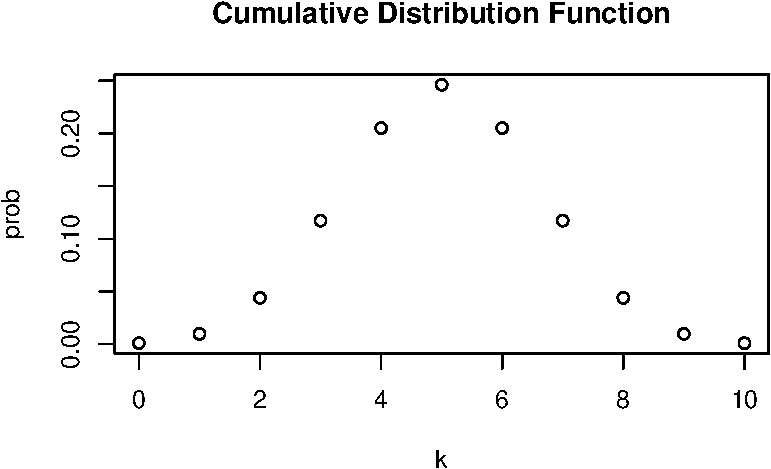
\includegraphics{bookdown-demo_files/figure-latex/unnamed-chunk-22-1} \end{center}

We find that, as \(n\) increases, the distribution of \(\hat\beta_1\)
concentrates around its mean, i.e.~its variance decreases. Put
differently, the likelihood of observering estimates close to the true
value of \(\beta_1 = 3.5\) grows as we increase the sample size. The
same can be observed for the distribution of \(\hat\beta_0\).

Furthermore, (4.1) reveals that the variance of the OLS estimator for
\(\beta_1\) decreases as the variance of the \(X_i\) increases. In other
words, as we increase the amount of information provided by the
regressor, that is increasing \(Var(X)\), which is used to estimate
\(\beta_1\), we are more confident that the estimate is close to the
true value (i.e. \(Var(\hat\beta_1)\) decreases). We can visuzalize this
by reproducing figure 4.6 from the book. To do this, we sample \(100\)
observations \((X,Y)\) from a bivariate normal distribution with
\(E(X)=E(Y)=5\), \(Var(X)=Var(Y)=5\) and \(Cov(X,Y)=4\). Formally, this
is written down as

\begin{align}
  \begin{pmatrix}
    X \\
    Y \\
  \end{pmatrix}
  \sim & \ \mathcal{N} 
  \left(
    \begin{pmatrix}
      5 \\
      5 \\
    \end{pmatrix}, \ 
    \begin{pmatrix}
      5 & 4 \\
      4 & 5 \\
    \end{pmatrix}
  \right). \tag{4.3}
\end{align}

To carry out the random sampling, we make use of the function
\texttt{mvtnorm} from the package \texttt{MASS}, see \texttt{?mvtnorm}.
Next, we use the \texttt{subset} function to split the sample into two
subsets such that the first set, \texttt{set1}, consists of observations
that fulfill the condition \(\lvert X - \overline{X} \rvert > 1\) and
the second set, \texttt{set2}, includes the remainder of the sample. We
then plot both sets and use different colors to make them
distinguishable.

\begin{Shaded}
\begin{Highlighting}[]
\CommentTok{# load the MASS package}
\KeywordTok{library}\NormalTok{(MASS)}

\CommentTok{# set random seed for reproducibility}
\KeywordTok{set.seed}\NormalTok{(}\DecValTok{4}\NormalTok{)}

\CommentTok{# simulate bivarite normal data}
\NormalTok{bvndata <-}\StringTok{ }\KeywordTok{mvrnorm}\NormalTok{(}\DecValTok{100}\NormalTok{, }
                \DataTypeTok{mu =} \KeywordTok{c}\NormalTok{(}\DecValTok{5}\NormalTok{,}\DecValTok{5}\NormalTok{), }
                \DataTypeTok{Sigma =} \KeywordTok{cbind}\NormalTok{(}\KeywordTok{c}\NormalTok{(}\DecValTok{5}\NormalTok{,}\DecValTok{4}\NormalTok{),}\KeywordTok{c}\NormalTok{(}\DecValTok{4}\NormalTok{,}\DecValTok{5}\NormalTok{))}
\NormalTok{                ) }

\CommentTok{# assign column names / convert to data.frame}
\KeywordTok{colnames}\NormalTok{(bvndata) <-}\StringTok{ }\KeywordTok{c}\NormalTok{(}\StringTok{"X"}\NormalTok{,}\StringTok{"Y"}\NormalTok{)}
\NormalTok{bvndata <-}\StringTok{ }\KeywordTok{as.data.frame}\NormalTok{(bvndata)}

\CommentTok{# subset the data}
\NormalTok{set1 <-}\StringTok{ }\KeywordTok{subset}\NormalTok{(bvndata, }\KeywordTok{abs}\NormalTok{(}\KeywordTok{mean}\NormalTok{(X) }\OperatorTok{-}\StringTok{ }\NormalTok{X) }\OperatorTok{>}\StringTok{ }\DecValTok{1}\NormalTok{)}
\NormalTok{set2 <-}\StringTok{ }\KeywordTok{subset}\NormalTok{(bvndata, }\KeywordTok{abs}\NormalTok{(}\KeywordTok{mean}\NormalTok{(X) }\OperatorTok{-}\StringTok{ }\NormalTok{X) }\OperatorTok{<=}\StringTok{ }\DecValTok{1}\NormalTok{)}

\CommentTok{# plot both sets}
\KeywordTok{plot}\NormalTok{(set1, }\DataTypeTok{xlab =} \StringTok{"X"}\NormalTok{, }\DataTypeTok{ylab =} \StringTok{"Y"}\NormalTok{, }\DataTypeTok{pch =} \DecValTok{19}\NormalTok{)}
\KeywordTok{points}\NormalTok{(set2, }\DataTypeTok{col =} \StringTok{"steelblue"}\NormalTok{, }\DataTypeTok{pch =} \DecValTok{19}\NormalTok{)}
\end{Highlighting}
\end{Shaded}

\begin{center}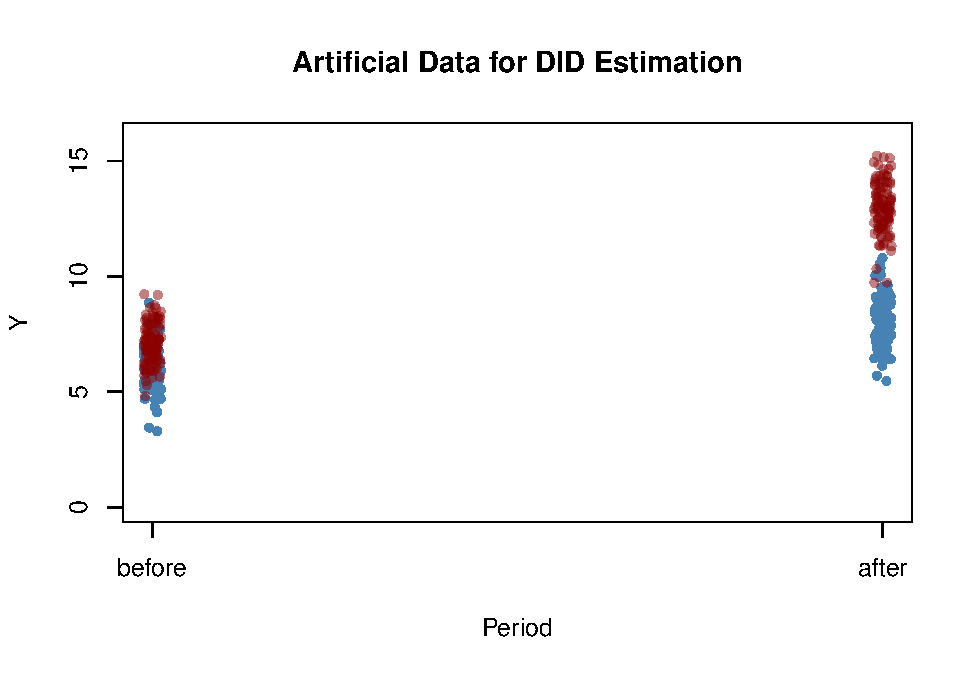
\includegraphics{bookdown-demo_files/figure-latex/unnamed-chunk-23-1} \end{center}

It is clear that observations that are close to the sample average of
the \(X_i\) have less variance than those that are farther away. Now, if
we were to draw a line as accurately as possible through either of the
two sets it is obvious that choosing the observations indicated by the
black dots, i.e.~using the set of observations which has larger variance
than the blue ones, would result in a more precise line. Now, let us use
OLS to estimate and draw the regression lines for both sets of
observations.

\begin{Shaded}
\begin{Highlighting}[]
\CommentTok{# estimate both regression lines}
\NormalTok{lm.set1 <-}\StringTok{ }\KeywordTok{lm}\NormalTok{(Y }\OperatorTok{~}\StringTok{ }\NormalTok{X, }\DataTypeTok{data =}\NormalTok{ set1)}
\NormalTok{lm.set2 <-}\StringTok{ }\KeywordTok{lm}\NormalTok{(Y }\OperatorTok{~}\StringTok{ }\NormalTok{X, }\DataTypeTok{data =}\NormalTok{ set2)}

\CommentTok{# add both lines to the plot}
\KeywordTok{abline}\NormalTok{(lm.set1, }\DataTypeTok{col=}\StringTok{"green"}\NormalTok{)}
\KeywordTok{abline}\NormalTok{(lm.set2, }\DataTypeTok{col=}\StringTok{"red"}\NormalTok{)}
\end{Highlighting}
\end{Shaded}

\begin{center}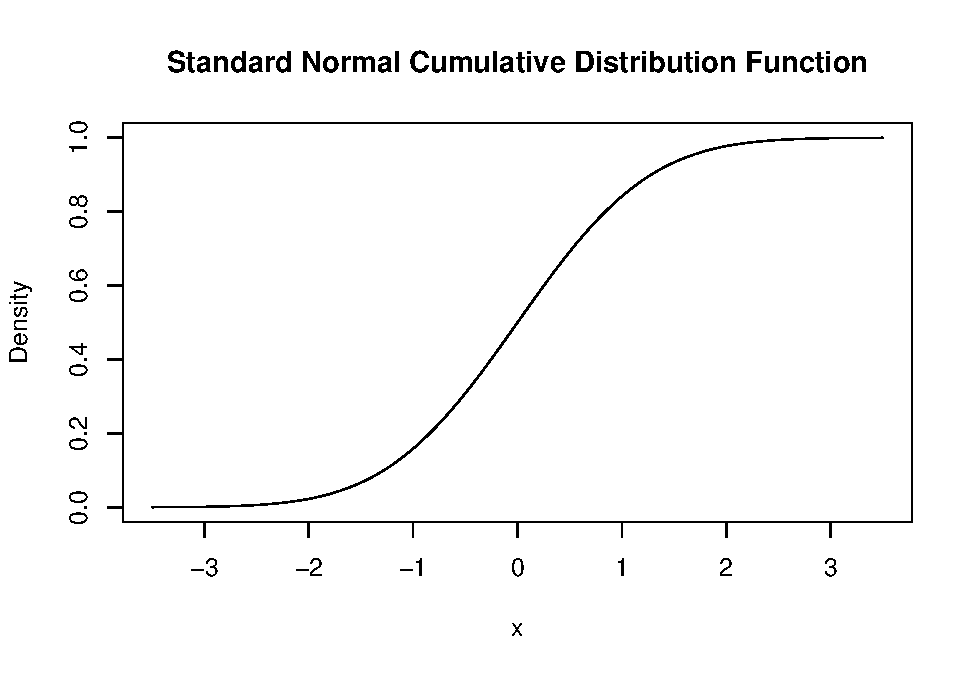
\includegraphics{bookdown-demo_files/figure-latex/unnamed-chunk-24-1} \end{center}

Evidently, the green regression line does far better in describing data
sampled from the bivariate normal distribution stated in (4.3) than the
red line.

\chapter{Methods}\label{methods}

We describe our methods in this chapter.

\chapter{Applications}\label{applications}

Some \emph{significant} applications are demonstrated in this chapter.

\section{Example one}\label{example-one}

\section{Example two}\label{example-two}

\chapter{Final Words}\label{final-words}

We have finished a nice book.

\bibliography{packages.bib,book.bib}


\end{document}
